\documentclass{crescendorepchap}
%**********************************************************
%
% Bibliography support
%
%**********************************************************
%\def\@reportno{YY--NN}		% default report no.
%\def\reportno#1{\gdef\@reportno{#1}}
\usepackage[nounderscore]{syntax}
\usepackage{capt-of}
\usepackage{multirow}
\usepackage{fancyhdr}
\usepackage{longtable}
\usepackage{vdmlisting}
\newcommand{\bthisbibliography}[1]{\chapter*{References}%
   \begin {list} {}%
     {\settowidth {\labelwidth} {[#1]XX}%
      \setlength {\leftmargin} {\labelwidth}%
      \addtolength{\leftmargin} {\labelsep}%
      \setlength {\parsep} {1ex}%
      \setlength {\itemsep} {2ex}%
     }
  }
\newcommand{\ethisbibliography}{\end{list}}
\newcommand{\refitem}[2]
  {\bibitem[#1]{#2}}

\newcommand{\back}{$\setminus$}
\newcommand{\RuleTarget}[1]{\hypertarget{rule:#1}{}}
\newcommand{\Ruledef}[2]
{
  \RuleTarget{#1}\Rule{#1}{#2}%
  }
\newcommand{\Ruleref}[1]{
  \hyperlink{rule:#1}{#1}}
\newcommand{\Lit}[1]{`{\tt #1}\Quote}
\newcommand{\Rule}[2]{
  \begin{quote}\begin{tabbing}
    #1\index{#1}\ \ \= = \ \ \= #2  ; %    Adds production rule to index

  \end{tabbing}\end{quote}
  }
%%%%%%%%%%%%%%%%%%%%%%%%%%%%%%%%%%%%%%%%%%%%%%%%%%%%%%%%%%%%%
%%% Model transformation rule box
%%%%%%%%%%%%%%%%%%%%%%%%%%%%%%%%%%%%%%%%%%%%%%%%%%%%%%%%%%%%%
\newcounter{formationRule}
\setcounter{formationRule}{0}
\newenvironment{formationRule}
%{\refstepcounter{formationRule}\vspace{10pt}\par\noindent
%Exercise \theformationRule
%\begin{itshape}\par\noindent\vspace{10pt}}%
%{\end{itshape}\vspace{10pt}\par}
{%
\refstepcounter{formationRule}
%increment
%\addtocounter{transformationRuleCounter}{1}%
%\ctf{}%
%\labelformat{formationRule}{\value{formationRule}}
\begin{center}%
\begin{tabular}{ | p{10cm} |}\hline%
\textbf{Transformation Rule \theformationRule}

}
{
\\
    \hline
    \end{tabular}
\end{center}

}
\newcommand{\kw}[1]{{\textbf\ttfamily #1}}
\newcommand{\SeqPt}[1]{\{\ #1\ \}}
\newcommand{\lfeed}{\\ \> \>}
\newcommand{\dsepl}{\ $|$\ }
\newcommand{\dsep}{\\ \> $|$ \>}
\newcommand{\Lop}[1]{`{\sf #1}\Quote}
\newcommand{\blankline}{\vspace{\baselineskip}}
\newcommand{\Brack}[1]{(\ #1\ )}
\newcommand{\nmk}{\footnotemark}
\newcommand{\ntext}[1]{\footnotetext{{\bf Note: } #1}}
\newlength{\kwlen}
\newcommand{\Keyw}[1]{\settowidth{\kwlen}{\tt #1}\makebox[\kwlen][l]{\sf
    #1}}
\newcommand{\keyw}[1]{{\sf #1}}
\newcommand{\vdmkeyw}[1]{{\bf\ttfamily #1}}

\newcommand{\id}[1]{{\tt #1}}
\newcommand{\metaiv}[1]{\begin{alltt}\input{#1}\end{alltt}}

\newcommand{\OptPt}[1]{[\ #1\ ]}
\newcommand{\MAP}[2]{\kw{map }#1\kw{ to }#2}
\newcommand{\INMAP}[2]{\kw{inmap }#1\kw{ to }#2}
\newcommand{\SEQ}[1]{\kw{seq of }#1}
\newcommand{\NSEQ}[1]{\kw{seq1 of }#1}
\newcommand{\SET}[1]{\kw{set of }#1}
\newcommand{\PROD}[2]{#1 * #2}
\newcommand{\TO}[2]{$#1 \To #2$}
\newcommand{\FUN}[2]{#1 \To #2}
\newcommand{\PUBLIC}{\ifthenelse{\boolean{VDMpp}}{public\mbox{}}{\mbox{}}}
\newcommand{\PRIVATE}{\ifthenelse{\boolean{VDMpp}}{private}{\mbox{}}}
\newcommand{\PROTECTED}{\ifthenelse{\boolean{VDMpp}}{protected}{\mbox{}}}

\pagestyle{fancy}
\fancyhead{}
\fancyhead[LO]{\leftmark}
\fancyhead[RE]{Crescendo Tool Support: User Manual}
\fancyhead[RO,LE]{\resizebox{0.05\textwidth}{!}{
\includegraphics{crescendo_logo_512}}}
\fancyfoot[C]{\thepage}

\usepackage{makeidx}

\usepackage{graphicx, color}

% definition of VDM++, JavaCC, JJTree, JTB, ANTLR and SableCC for listings
\newcommand{\NL}{\mbox{}\\ \vspace*{-5mm}}
\usepackage{listings}
\usepackage{listingsDCL}
\newcommand{\url}[1]{\texttt{#1}}
%\usepackage{vdmsl-2e}
\usepackage{hyperref}

\usepackage{times}
\usepackage{color}

%\include{ifad}
%\include{graphics}
\usepackage{cite}
\usepackage{alltt}
%\usepackage{fancyhdr}
\renewcommand{\topfraction}{0.9}
\renewcommand{\textfraction}{0.05}
\renewcommand{\floatpagefraction}{0.9}
\makeindex

\begin{document}

\frontmatter

\title{Crescendo Tool Support: User Manual \\{\large Version 2.0.0}}
\author{Peter Gorm Larsen, Kenneth Lausdahl, Joey Coleman and Sune Wolff \\
Aarhus University, Department of Engineering\\
Finlandsgade 22, DK-8200 Aarhus N, Denmark\\[5mm]
Christian Kleijn and Frank Groen\\
Controllab Products B.V.\\
Hengelosestraat 500, 7521 AN Enschede, The Netherlands
}

\date{November 2013}

\reportno{TR-001}

\maketitle


\textbf{Document history}

\begin{tabular}{|l|l|l|l|}\hline
Month   & Year & Version & Version of Crescendo.exe \\ \hline
December& 2012 & 1       & 1.1.8 (then called DESTECS)  \\ \hline
November& 2013 & 2       & 2.0.0 \\ \hline
\end{tabular}

\tableofcontents

\begin{abstract}
This document is the user manual for the Crescendo Integrated
Development Environment (IDE) version 2.0.0 enabling collaborative
analysis of models written in the Discrete-Event (DE) formalism VDM
and the Continuous-Time (CT) formalism bond graphs. The specific
dialect of VDM is called VDM Real Time (VDM-RT) and it is supported by
the Overture tool whereas the bond graph formalism is supported by the
tool called 20-sim.  Both the Crescendo as well as the Overture tool
is built on top of the Eclipse platform.
\end{abstract}

\mainmatter

\chapter{Introduction}

\section{What is the Crescendo Tool?}\label{sec:crescendointro}

The Crescendo tool was originally called the DESTECS tool since it was produced in the European research project called DESTECS (see Section~\ref{sec:destecs} below). It supports collaborative modelling and simulation called \emph{co-simulation}. 

\section{What was the DESTECS Project?}\label{sec:destecs}

The DESTECS (Design Support and Tooling for Embedded Control
Software)\footnote{See \url{www.destecs.org}.} project had a
consortium of research groups and companies working on the challenge
of developing fault-tolerant embedded systems \cite{Broenink&10}. The
consortium focussed on developing design methods and tools that
bridge the gap between the disciplines involved in designing an
embedded system: systems, control, mechanical and software
engineering, for example.  DESTECS aimed to develop methods and tools
that that combine Continuous-Time (CT) models with Discrete-Event (DE)
controller models through co-simulation to allow multi-disciplinary
modelling, including modelling of faults and fault tolerance
mechanisms. The analysis of these effects at every stage in a design
process will help to build more dependable real-time embedded systems. The DE modelling is carried out using the Vienna Development Method and its support tool Overture (see Section~\ref{sec:vdm} below). The CT modelling is carried out using bond graphs and its support tool 20-sim (see Section~\ref{sec:bond} below).

\section{What is the Vienna Development Method?} \label{sec:vdm}

The Vienna Development Method (VDM) is one of the longest established
model-oriented formal methods for the development of computer-based
systems and software
\cite{Bjorner&78,Jones90a,Fitzgerald&08c}. It consists of a
group of mathematically well-founded languages for expressing system
models during early design stages, before expensive implementation
commitments are made. VDM has a strong record of industrial
application, in many cases has been used
by practitioners who were not specialists in
the underlying formalism or logic
\cite{Larsen&96b,Clement&99,Kurita&09}. Experience with the method
suggests that the effort expended on formal modelling and analysis can
be recovered in reduced rework costs arising from design errors.

VDM models are expressed in a specification language (VDM-SL) which
supports the description of data and functionality
\cite{ISOVDM96a,Fitzgerald&98b,Fitzgerald&09}. Data are defined by
means of types built using constructors that define structured data
and collections such as sets, sequences and mappings from basic values
such as Booleans and natural numbers. These types are very abstract,
allowing you to add any relevant constraints using data type
invariants. Functionality is defined in terms of operations over these
data types. Operations can be defined implicitly by preconditions and
postconditions that characterize their behavior, or explicitly by
means of specific algorithms. An extension of VDM-SL, called VDM++,
supports object-oriented structuring of models and permits direct
modelling of concurrency \cite{Fitzgerald&05}. A further extension
to VDM++, called VDM Real Time (VDM-RT\footnote{Formerly called VDM In a
Constrained Environment (VICE).}), includes support for discrete
time models \cite{Mukherjee&00,Verhoef&06b}. All
three VDM dialects are supported by Overture.

\section{What are Bond Graphs?}\label{sec:bond}

Bond graphs are directed graphs in which the vertices are submodels
and the edges, called \textit{bonds}, denote the ideal (or idealised)
exchange of energy. Entry points of submodels are called
\textit{ports}. The exchange of energy through a port ($p$) is always
described by two implicit variables, effort ($p.e$) and flow
($p.f$). The product of these variables is the amount of energy that
passes through the port. The meaning of these two variables depends on
the physical domain (examples include voltage and current, and force
and velocity).

The 20-sim tool supports the creation and simulation of models that
can be represented in a variety of forms, including basic bond graphs;
collections of differential equations describing the behaviour of
nodes; and iconic diagram. Although the tool is commercial, all the
model libraries are open source. The package supports mixed-mode
integration techniques to allow the modelling and simulation of
computer controlled \textit{physical systems} that contain
Continuous-Time as well as Discrete-Event elements. The level of
complexity of many modern controllers means that discrete-event
elements are better modelled using a rich formalism such as VDM. The
20-sim package supports the connection of external software both for
model construction and simulation~(Discrete-Event, Continuous-Time or
hybrid), and this connection is exploited in providing support for
co-simulation.

\section{Related Tools}\label{sec:toolsIntro}

\subsection{Overture}

\subsection{Crescendo}

\subsection{Symphony}

\section{Structure of this User Manual}\label{sec:structure}

This user manual explains how to use the Crescendo IDE for developing collaborating models
 (co-models) and analyse them. In essence it is structured in 2 parts: The first part provides the basics for getting started using the Crescendo tool and the second part act as a reference manual for the Crescendo tool. The first part contains Chapter~\ref{chap:introconcepts} introducing the basic Crescendo concepts\footnote{Appendix~\ref{app:Glossary} provides a complete list of the Crescendo common concepts.};
Chapter~\ref{chap:getting} explaning how to get hold of the software; and finally
Chapter~\ref{chap:gettingstarted} with information about how to quickly get started using the Crescendo tool with existing models that can be imported directly. Afterwards the second part also contains four chapters explaining the main possibilities in the Crescendo tool. Chapter~\ref{chap:basic} explains the different views in the Crescendo tool, its editors and its way of handling projects. Afterwards, Chapter~\ref{chap:cosim} explains the co-simulation possibilities. This is followed by Chapter~\ref{chap:DSE} which provides information about how co-simulation can be extended with exploring the candidate design space. Finally this part is completed in Chapter~\ref{chap:postana} explaining the post-analysis possibilities in particular relevant in an exploration setting.

\chapter{Basic Crescendo Concepts}\label{chap:introconcepts}

The Crescendo tool allows you to define and run a co-simulation. To get a
basic understanding of the tool we first need to define some concepts.
We will use a popular description of these concepts that might not
be completely correct but will, hopefully, enhance the understanding of
beginning Crescendo users.

\section{Models}

It starts with models. Models are a more or less abstract representation
of a system or component of interest. In Crescendo we use
\emph{Continuous-Time models (CT models)}~and \emph{Discrete-Event
models (DE models)}.~CT models are models that describe
real physical systems. These models describe the behaviour of physical
systems at any desired time. DE models typically describe
computer systems that run at predetermined time steps. Between these
time steps nothing happens.

\section{Simulation}

Continuous-Time models can be created and simulated in 20-sim. This tool
will simulate CT models with as many small time steps as
required to get accurate results. Sometime the accuracy is violated. The
tool will then step back and use smaller time steps until the required
accuracy is met. This is called a \emph{Continuous-Time simulation}. A
Continuous-Time simulation is therefore always characterized by the
accuracy of the simulation and the time steps taken.~Discrete-Event
models can be created and simulated in Overture/VDM. This tool will simulate
Discrete-Event models with predetermined discrete time steps. This is
called a \emph{Discrete-Event simulation}. There is no accuracy issues
involved and therefore no backstepping is required.

The properties of a model~that affects its behaviour, but which remains
constant during a simulation are called \emph{parameters}. Examples of
parameters are the \texttt{height} of a watertank with varying waterlevel or
the \texttt{mass} of a car with varying~speed. A \emph{variable} is a
property~of a model that may change during a given simulation. Examples
of variables are the varying \texttt{waterlevel} of a watertank~or the
varying \texttt{speed} of a car.

\section{Co-Simulation}

A \emph{co-simulation} is a combined simulation of a Continuous-Time
model and a Discrete-Event model in separate tools. The Crescendo tool
allows you to run Discrete-Event models in VDM and Continuous-Time
models in 20-sim and exchange information between VDM and 20-sim during
run time. Because the notion of a model in a co-simulation may lead
to misinterpretations, we will use the following definitions:

\begin{description}
\item[constituent model:] the CT submodel or the
  DE submodel of a co-simulation.
\item[co-model:] a model comprising two constituent models (a
  DE submodel and a CT submodel).
\end{description}

\section{Contract}

The description of the communication between the constituent models of a
co-model is called the \emph{contract}. A contract typically describes
the variables that are shared between the Continuous-Time model and the
Discrete-Event model. An example of a \emph{shared variable} is the
\texttt{waterlevel} that is calculated in the Continuous-Time model and sent to
the Discrete-Event model where it is used to calculate the response of a
water level controller.

In most cases a Continuous-Time model and a Discrete-Event model will
use similar parameters. For the watertank example such a parameter may
be the maximum water level. In the Continuous-Time model this parameter
indicates the height at which a sensor is placed and in the Discrete-Event
model this parameter may indicate a property of the water level
controller. To prevent different values to be used in the
Continuous-Time model and Discrete-Event model, we may share this
parameter in the contract. This is called a \emph{shared design
parameter}.

\chapter{Getting Hold of the Software}\label{chap:getting}

\section{Requirements}

The Crescendo tool suite can be downloaded as a single installation
package from the Crescendo website. The package contains a
full installation for Overture/VDM, 20-sim and the
Crescendo tools. Overture/VDM and the Crescendo tools are open source tools and
will run on any computer. However, 20-sim is a commerical tool that will run as a
viewer on any computer. If you want to build your own models in 20-sim
and store them, you will need a license (see Section~\ref{sec:install}). In order to install to package of the Crescendo package you need to have:

\begin{itemize}
\item
  Windows platform (XP / Vista / 7 / 8)
\item At least
  256 MB memory
\item At least
  200 MB free disk space
\item An
  x86 compatible CPU
\end{itemize}

\section{Installation}\label{sec:install}

\subsection{Combined Installer}

First-time users are advised to use the combined installer that will
install the Crescendo tool and that will also include the Overture/VDM features and the 20-sim tool on your computer. You can
download the installer from the Crescendo website:

\begin{quote}
\url{http://www.crescendotool.org}
\end{quote}

During installation the main installer will pause. A second installer
will then guide you through the installation of 20-sim. Once 20-sim is
installed, the Crescendo installer will continue.

\subsection{License}

Both VDM and the Crescendo tools are open source and do not require an
additional license. 20-sim is a commercial tool that will run in
Viewer mode on any computer. This means that you
can only run and edit models! If you want to save model changes, you will need
a license. You can send an email to
Controllab \url{mailto://info@controllab.nl} to get a trial license.

\subsection{Manuals}

\begin{description}
\item[VDM:] To help you work with VDM the VDM language manual~\cite{Larsen&13b} and the Overture user guide~\cite{Larsen&13a}\footnote{Both of these and more manuals can be found at
  \url{http://overturetool.org/?q=Documentation}.}.
\item[20-sim:] To help you work with 20-sim, you can visit the
  website~\cite{20sim} or look at the reference
  manual~\cite{Kleijn09}\footnote{See also
    \url{http://www.20sim.com/support/movies.html}
    or~\url{http://www.20sim.com/downloads/files/20sim43GettingStartedManual.pdf}.}.
\end{description}

\section{20-sim Standalone}

The Crescendo installer will install the 20-sim Viewer on your computer.
The 20-sim Viewer will allow you to run and edit all the Crescendo example
models, but does not allow you to save them. When 20-sim is openened,
the license dialog will be opened.

\begin{figure}[htbp]
\centering
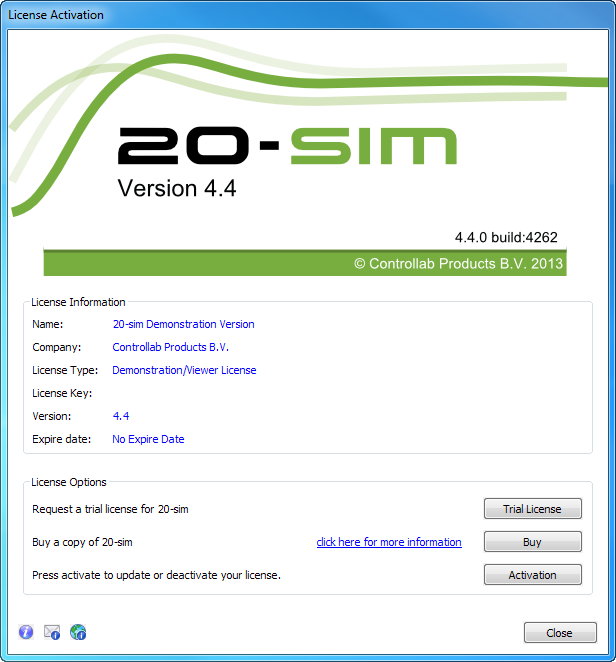
\includegraphics[width=.4\textwidth]{images/20simLicense.png}
\caption{License for 20-sim.}
\end{figure}

\begin{itemize}
\item
  You have to click the \emph{Close} button to continue.
\end{itemize}

Unless you have purchased a license during model editing and
simulation, the 20-sim Viewer will annoy you with a message:

\begin{figure}[htbp]
\centering
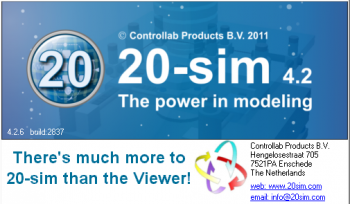
\includegraphics[width=.6\textwidth]{images/20simViewer.png}
\caption{Message if you do not have a license for 20-sim.}
\end{figure}

\begin{itemize}
\item
  You have to \emph{click on top} of this message to continue.
\end{itemize}

If you feel the Viewer is too annoying or want to store models, you have
to ask Controllab for trial license.

\chapter{Quick Start with Crescendo} \label{chap:gettingstarted}

To help you get started with Crescendo this chapter gives you step
by step instructions how to configure the software, get a basic
\texttt{WaterTankPeriodic} example running and create your own simple project.


\section{Opening Crescendo}

\begin{itemize}
\item
  \textbf{Open Crescendo} from the \textbf{start menu}.
You will see a splash screen when the program opens and a dialog
prompting you to give a location for the workspace as in Figure~\ref{fig:wsloc}.
\end{itemize}

\begin{figure}[htbp]
\centering
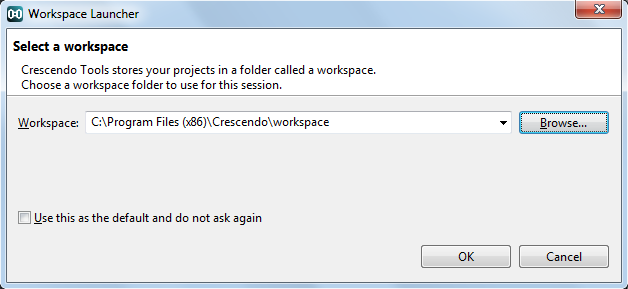
\includegraphics[width=.8\textwidth]{images/DestecsWorkspaceLocation.png}
\caption{The Crescendo Workspace Location Screen.\label{fig:wsloc}}
\end{figure}

\begin{itemize}
\item
  \textbf{Enter a location} where you have both read and write access.
The program should respond by opening with a welcome screen as shown in Figure~\ref{fig:welcome}.
\end{itemize}

\begin{figure}[htbp]
\centering
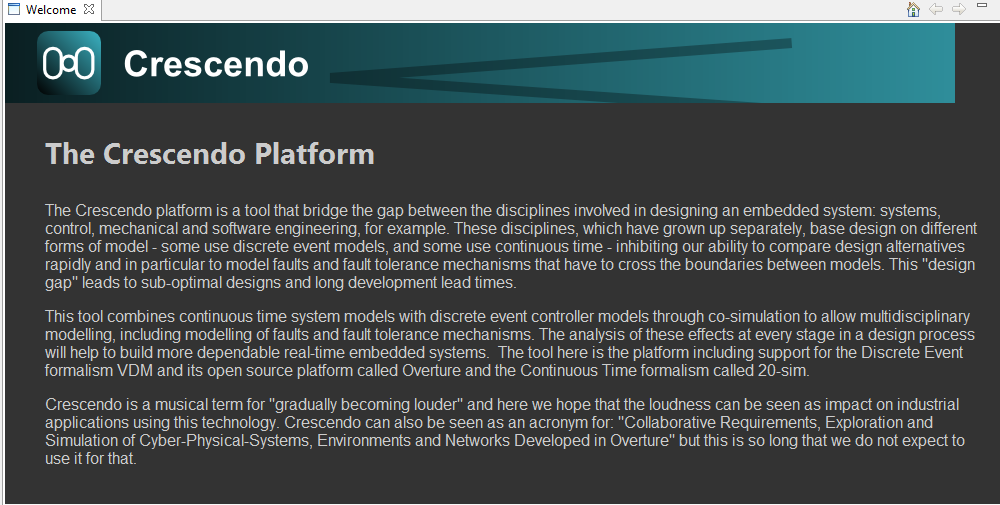
\includegraphics[width=.8\textwidth]{images/DestecsSplash.png}
\caption{The Crescendo Welcome Screen.\label{fig:welcome}}
\end{figure}

When the welcome screen is closed the standard Crescendo perspective as shown in Figure~\ref{fig:DestecsStartScreen} with different views explained further in Chapter~\ref{chap:basic}.

\section{Opening a Project}

\begin{itemize}
\item
  From the \emph{File} menu choose ``\emph{File} and then \emph{Import}''.
\item
  Select ``\emph{General and Existing Projects into Workspace}''
  and click \emph{Next} and get a window similar to Figure~\ref{fig:importex}.
\item
  \emph{Crescendo Examples} and select at least the
  \texttt{WatertankPeriodic} example.
\item
  Click \emph{Finish} to import the selected project(s).
\end{itemize}

\begin{figure}[htbp]
\centering
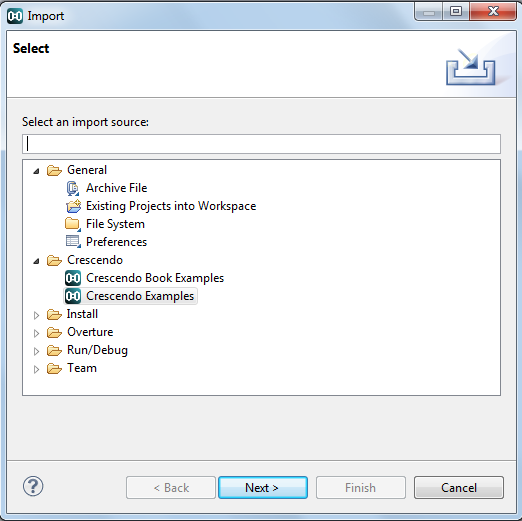
\includegraphics[width=.8\textwidth]{images/DestecsImportDialog.png}
\caption{Dialog for Importing Crescendo Examples\label{fig:importex}}
\end{figure}

\section{Running a Project}

Now (at least) the \texttt{WaterTankPeriodic} project should be visible.

\begin{itemize}
\item
  \textbf{Click on the WaterTankPeriodic} project entry to select it.
\item
  Press the \emph{Debug button}
  (if you have multiple
  projects loaded, you have to select the \texttt{Water\-Tank\-Periodic} project first, by
  clicking the black triangle at the right of the Debug button)
\end{itemize}

Now a co-simulation will start. The 20-sim editor (showing the
Continuous-Time model) will be opened as shown in
Figure~\ref{fig:watertankeditor}, the 20-sim Simulator (showing the
plot of the Continuous-Time part of the simulation) will be opened and
the 3D animator (showing an animation of the watertank) will be opened
as shown in Figure~\ref{fig:water3Dani}. In addition graphs for
selected variables during the simulation is shown as in
Figure~\ref{fig:watercosimplot}.

\begin{figure}[htbp]
\centering
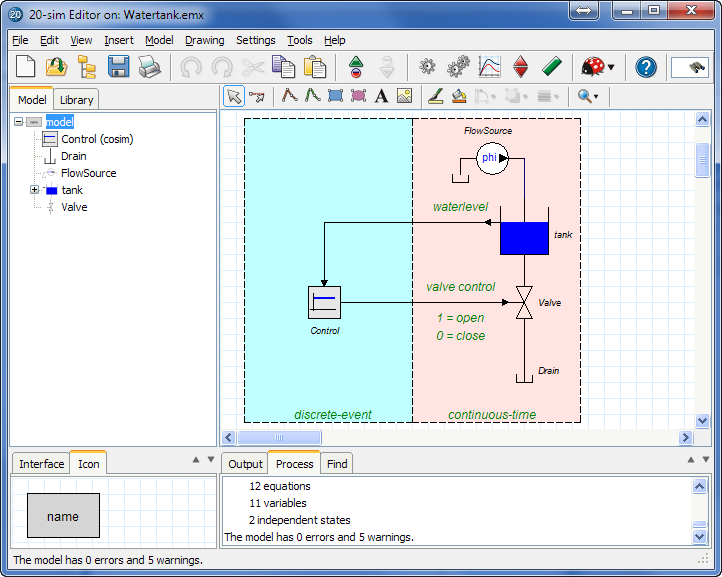
\includegraphics[width=.9\textwidth]{images/20simEditorWaterTank.png}
\caption{The 20-sim Editor contains the continuous-time \texttt{WaterTankPeriodic} model.\label{fig:watertankeditor}}
\end{figure}

\begin{figure}[htbp]
\centering
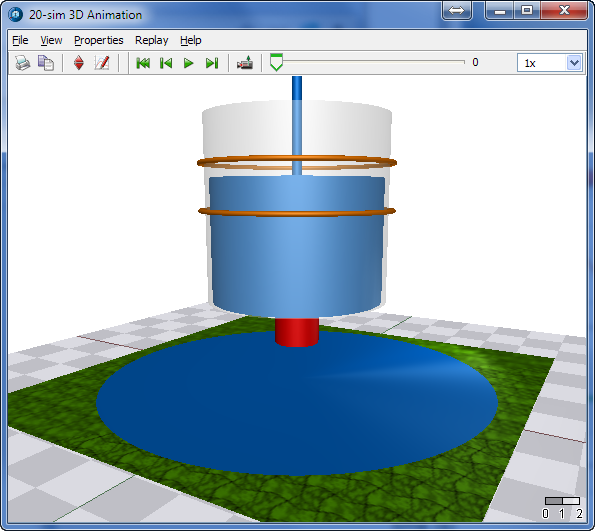
\includegraphics[width=.9\textwidth]{images/20simAnimationWaterTank.png}
\caption{20-sim can also show simulation results in a 3D animation.\label{fig:water3Dani}}
\end{figure}


\begin{figure}[htbp]
\centering
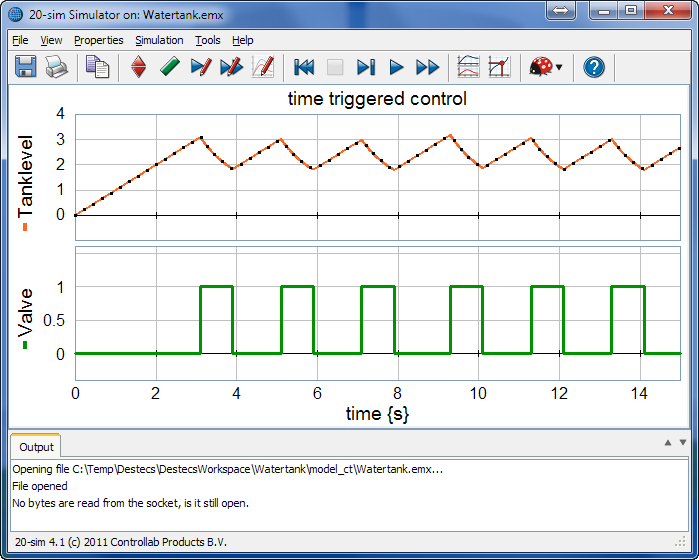
\includegraphics[width=.6\textwidth]{images/20simSimulatorWaterTank.png}
\caption{The 20-sim Simulator shows the co-simulated plots.\label{fig:watercosimplot}}
\end{figure}

\chapter{Editors and Management of Projects}\label{chap:basic}

\section{The Crescendo Workbench}\label{sec:crescendo}

Eclipse is an open source platform based around a workbench that
provides a common look and~feel to a large collection of extension
products. Thus, if a user is familiar with one Eclipse product, it will
generally be easy to start using a different product on the same
workbench. The Eclipse workbench consists of several panels known as
views as shown in Figure~\ref{fig:DestecsStartScreen}. 
A collection of panels is called a perspective. The figure below
shows the standard Crescendo perspective. The Crescendo perspective consists
of a set of views for managing Crescendo projects and viewing and editing
files in a project. Different perspectives are available in Crescendo
based on the task that you are doing. In the subsections below the different views of the standard Crescendo perspective will be presented.

\begin{figure}[htbp]
\centering
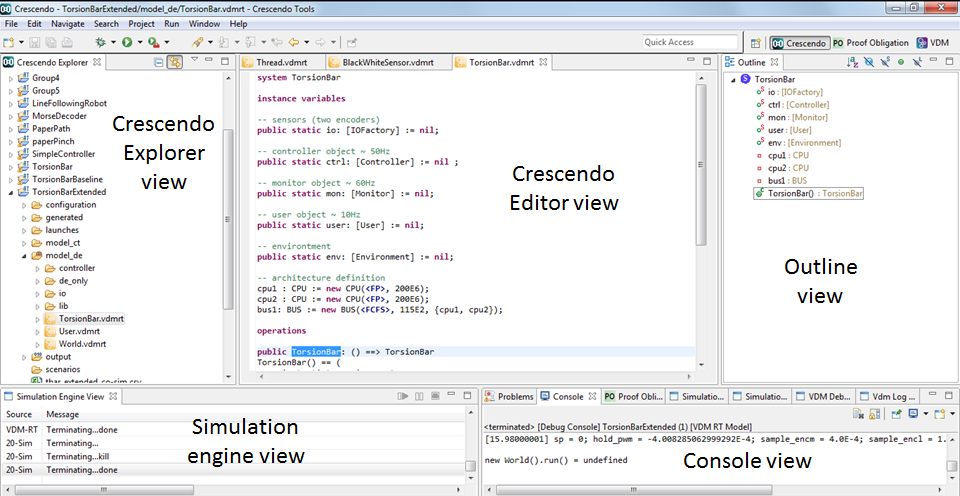
\includegraphics[width=.8\textwidth]{images/DestecsWorkbenchOutline.png}
\caption{Standard Crescendo Perspective.\label{fig:DestecsStartScreen}}
\end{figure}

\subsection{Explorer View}\label{subsec:explorer}

The Crescendo \emph{Explorer view} lets you create, select, import, export and delete Crescendo
projects and navigate between the files in these projects. It is also from this view that deleting existing files and
adding new files to existing projects is enabled. In Figure~\ref{fig:explorerview} the kind of contents inside one project is illustrated.

\begin{figure}[htbp]
\centering
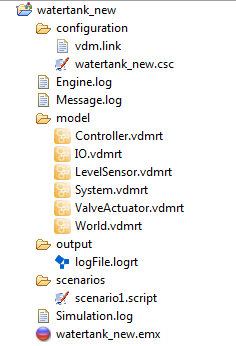
\includegraphics[width=.3\textwidth]{images/DestecsExplorer.png}
\caption{The Crescendo explorer view.\label{fig:explorerview}}
\end{figure}

\subsection{Editor View}\label{sec:editorview}

The Crescendo \emph{Editor View} allows you to edit VDM files, Contracts and Scenarios and it highlights the different keywords. Figure~\ref{fig:editorcontract1} showns how a Crescendo contract looks in the editor (and in a different pane a VDM-RT file).

\begin{figure}[htbp]
\centering
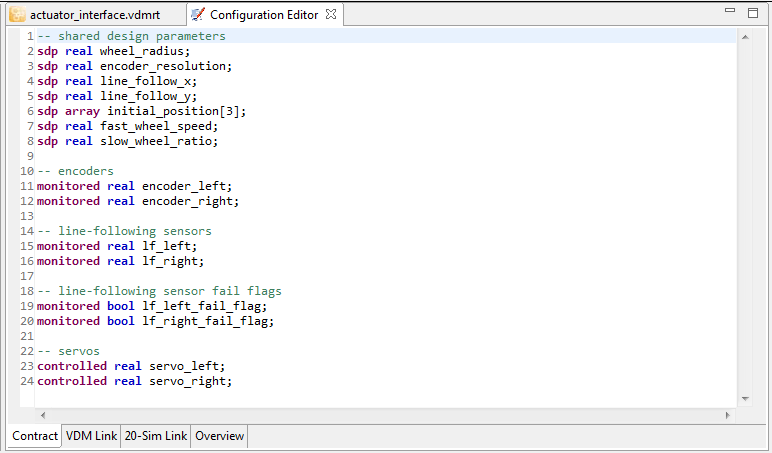
\includegraphics[width=.6\textwidth]{images/DestecsEditorNewContract.png}
\caption{The Editor View.\label{fig:editorcontract1}}
\end{figure}

\subsection{Outline View}

The Crescendo \emph{Outline view}, on the right hand side of Figure~\ref{fig:DestecsStartScreen}, presents
an outline of the file selected in the editor. This view displays any
declared VDM definitions such as their state components, values, types,
functions and operations. The type of the definitions are also shown in
the outline view. The Outline view is at the moment only available for
the VDM models of the system. In the case another type of file is
selected, the message: ``An outline is not available'' will be displayed. 
Figure~\ref{fig:outlineview} shows an extract of the outline of a class called \texttt{System}. 

\begin{figure}[htbp]
\centering
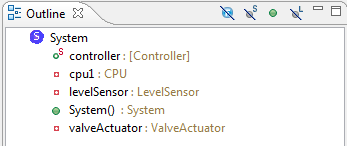
\includegraphics[width=.6\textwidth]{images/DestecsOutLineViewSystem.png}
\caption{The outline view showing the composition of the \texttt{System}
VDM-RT class.\label{fig:outlineview}}
\end{figure}

The
type of each definition is also shown in the view and the colour of
the icons in front of the names indicates the accessibility of each
definition. Red is
used for private definitions, yellow for protected definitions and
green for public definitions. Triangles are used for
type definitions, small squares are used for values, state components
and instance variables, functions and operations are represented by
larger circles and squares, permission predicates are shown with small
lock symbols and traces are shown with a
``\texttt{T}''. Functions have a small ``\texttt{F}'' superscript over the
icons and static definitions have a small ``\texttt{S}'' superscript.
Record types have a small arrow in front of the
icon, and if that is clicked the fields of the record can be seen.
Figure~\ref{fig:OutlineIcons} illustrates the different outline icons.
At the top of the view there are buttons to filter what is displayed,
for instance it is possible to hide non-public members.

\begin{figure}[!htb]
\begin{center}
  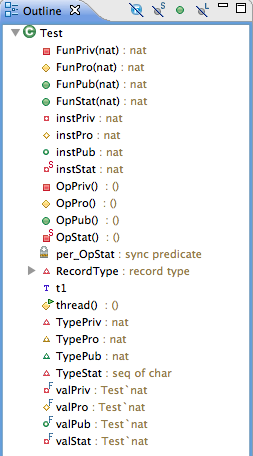
\includegraphics[width=2.5in]{images/OutlineIcons}
  \caption[labelInTOC]{Icons in the Outline View}
  \label{fig:OutlineIcons}
\end{center}
\end{figure}

Clicking on the name of a definition in the outline will navigate to
the definition and highlight the name in the Editor view (see Section~\ref{sec:editorview}).

\subsection{Simulation Engine View}

The Crescendo \emph{Simulation Engine View}, located in the lower left part of the
environment is showing the evolution of a co-simulation. This is done by
monitoring the interaction between the VDM-RT Discrete-Event simulation,
the 20-sim Continuous-Time simulation and the engine. This view has~two
columns, the first one is specifying the source of the message and the
second one the progress of a co-simulation in seconds and percentages of completion.
An extract of this is shown in Figure~\ref{fig:engineview}.

\begin{figure}[htbp]
\centering
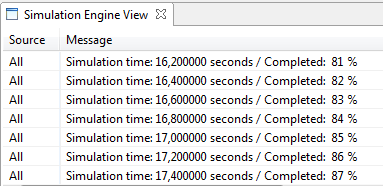
\includegraphics[width=.6\textwidth]{images/DestecsEngineView.png}
\caption{The Crescendo Simulation Engine view.\label{fig:engineview}}
\end{figure}

\subsection{Console View}

The Crescendo \emph{Colsole View}, located in the lower right part of the
environment is acting as a console showing any output from the DE-part of
the co-simulation.
An extract of this is shown in Figure~\ref{fig:consoleview}.

\begin{figure}[htbp]
\centering
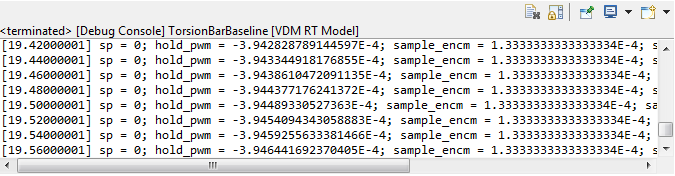
\includegraphics[width=.6\textwidth]{images/DestecsConsoleView.png}
\caption{The Crescendo Console view.\label{fig:consoleview}}
\end{figure}

%% \subsection{Simulation Messages View}

%% To the right of the Simulation Engine View, there is a view called the
%% Simulation Messages View from Figure~\ref{fig:simmes}. In this case different
%% messages coming specifically from the continuous or the discrete
%% simulation are shown. Each entry shows the source of the message, its
%% content and a timestamp.

%% \begin{figure}[htbp]
%% \centering
%% 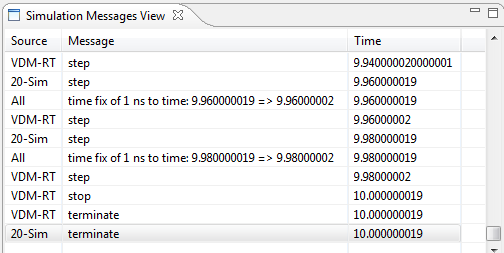
\includegraphics[width=.6\textwidth]{images/DestecsMessagesView.png}
%% \caption{The Simulation Message view.\label{fig:simmes}}
%% \end{figure}

%% \subsection{Simulation View}

%% A third view related to the simulation is the Simulation View, which
%% displays the evolution of~certain parameters specially relevant in the
%% co-simulation. As in the Simulation Messages View,~every message is
%% timestamped and ordered chronologically. This is illustrated in the
%% figure below.~There is a default arrangement of views in the
%% perspective, but they can be changed and then~restored to the default at
%% any time.

%% \begin{figure}[htbp]
%% \centering
%% 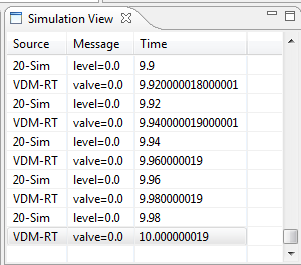
\includegraphics[width=.4\textwidth]{images/DestecsSimulationView.png}
%% \caption{The Simulation view.}
%% \end{figure}


\section{Handling Projects}

All data that is necessary for a co-simulation (e.g., models, contracts
etc.) is stored in a Crescendo project.~This section explains how to use
the Crescendo tool to manage projects. Step by step instructions~for
importing, exporting and creating projects will be given.

\subsection{Creating new Projects}

Follow these steps in order to create a new Crescendo project:

\begin{itemize}
\item
  Create a new project by choosing \emph{File} and \emph{New} and
  \emph{Project} and \emph{Crescendo project}.
\item
  Type in a project \texttt{name}.
\item
  Click the button ``\emph{Finish}'' (see Figure~\ref{fig:NewProject}).
\end{itemize}

\begin{figure}[htbp]
\centering
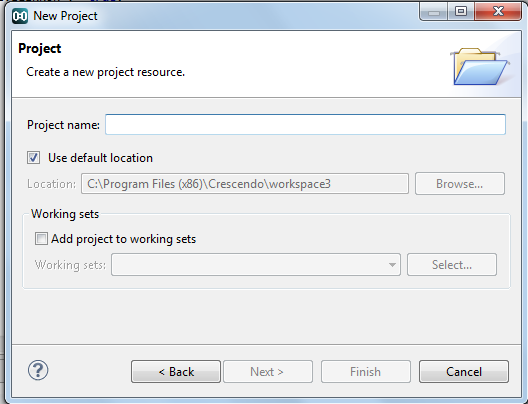
\includegraphics[width=.6\textwidth]{images/DestecsNewProject.png}
\caption{Create project dialog.\label{fig:NewProject}}
\end{figure}

You can create projects in the Crescendo tool. The highlighted project is
the project that is currently selected.

\subsection{Importing Projects}

Follow these steps in order to import an already existing Crescendo
project.

\begin{figure}[htbp]
\centering
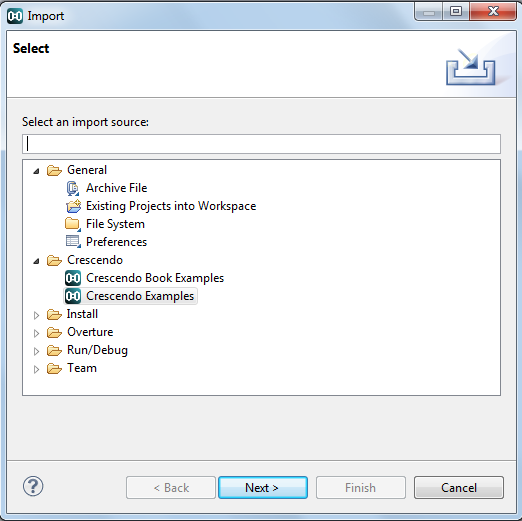
\includegraphics[width=.6\textwidth]{images/DestecsImportDialog.png}
\caption{Import project dialog.\label{fig:ImportDialogue}}
\end{figure}

\begin{itemize}
\item
  Right-click the \emph{Explorer View} (see Section~\ref{subsec:explorer} above)  and
  select \emph{Import.}
\item
  Select either the standard \emph{Crescendo} or the \emph{General - Existing Projects into
  Workspace} part. Using the \emph{Crescendo} one enables you to import the standard Crescendo examples or the examples used in the book about this \cite{Fitzgerald&13a}. Using the \emph{General} entry you can import anything else that has been produced by someone and exported for your use.
\item
  Click \emph{Next} to proceed.
\item
  If one of the \emph{Crescendo} options is taken a list of the potential projects to import will appear. Otherwise if the  \emph{General} one was selected you shall select the the radio button ``\emph{Select root directory}'' if the project
  is uncompressed. Otherwise select the the radio button ``\emph{Select archive
  file}'' if the project is contained in a compressed archive file. Afterwards, use
  the \emph{Browse} button to locate the project.
\item
  A compressed archive file may contain multiple projects. Select
  the projects that you want to import as shown in Figure~\ref{fig:importproject}.
\item
  Click the \emph{Finish} button. The imported project will appear on
  the Crescendo explorer view.
\end{itemize}

\begin{figure}[htbp]
\centering
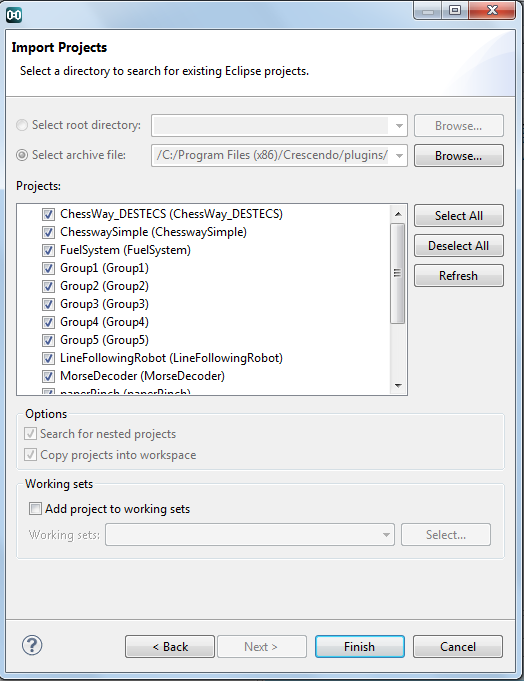
\includegraphics[width=.6\textwidth]{images/DestecsImportProject.png}
\caption{Import projects.\label{fig:importproject}}
\end{figure}


\subsection{Exporting Projects}

Follow these steps in order to export a Crescendo project:

\begin{itemize}
\item
  Right click on the target project and select \emph{Export}, followed
  by \emph{General} and \emph{Archive File}. See Figure~\ref{fig:export}
  for more details.
\item
  Click \emph{Next} to proceed.
\end{itemize}


\begin{figure}[htbp]
\centering
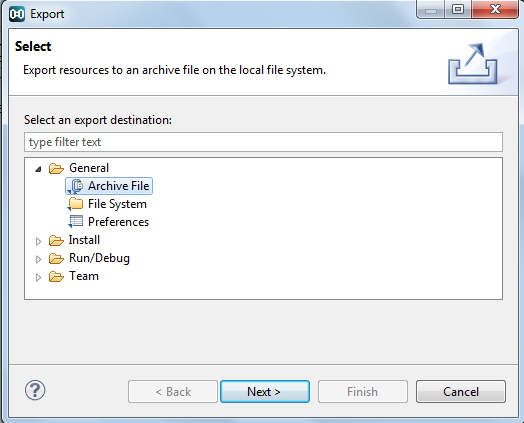
\includegraphics[width=.6\textwidth]{images/DestecsExportDialog.png}
\caption{Select an output format for the exporting process.\label{fig:export}}
\end{figure}

%% \section{Adding Models}

%% When you have created a new project, you have to define the
%% \emph{continuous-time model} and the
%% \emph{discrete-event model} that have to be coupled in
%% a co-simulation.

%% \subsection{Continuous-time model}

%% \begin{figure}[htbp]
%% \centering
%% 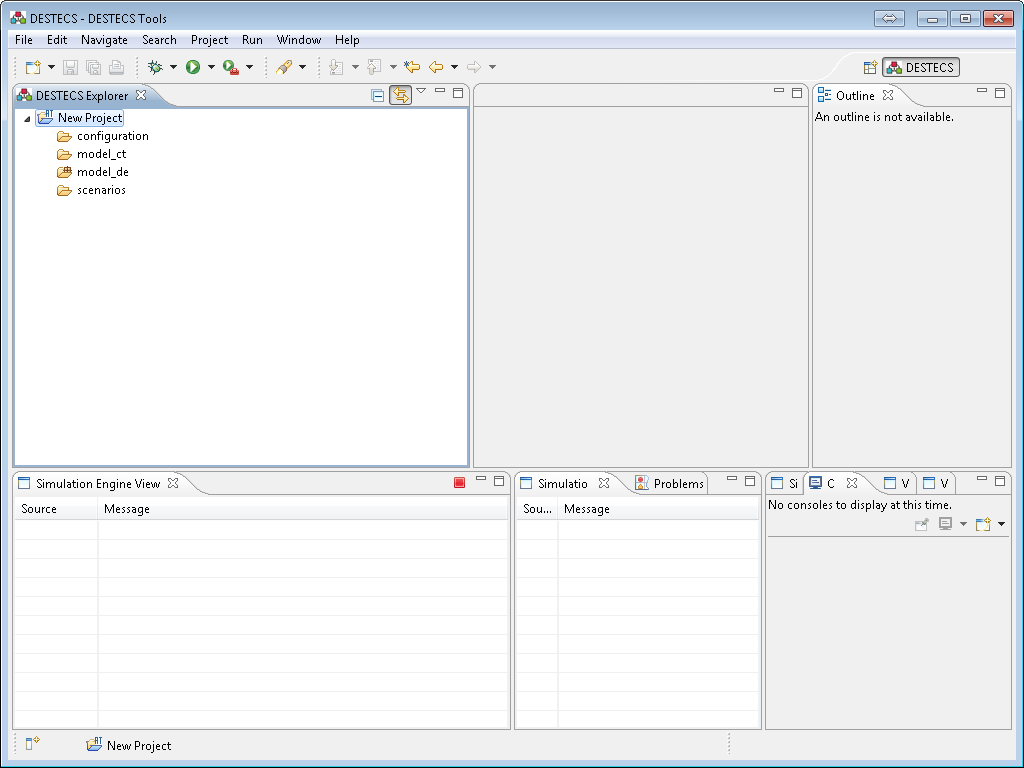
\includegraphics[width=.6\textwidth]{images/DestecsWorkbenchNewProject.png}
%% \caption{The project tree showing the CT and DT entries.}
%% \end{figure}

%% \begin{itemize}
%% \item
%%   Click on the \texttt{arrow} in front of the project name to expand the
%%   project tree.
%% \item
%%   Select the item~\texttt{model\_ct}.
%% \item
%%   Right-click and select \texttt{Import} - \texttt{File System}
%% \item
%%   From the \texttt{Import Dialog}, choose the '''directory '''that
%%   contains the \texttt{20-sim model}.
%% \end{itemize}

%% \begin{figure}[htbp]
%% \centering
%% 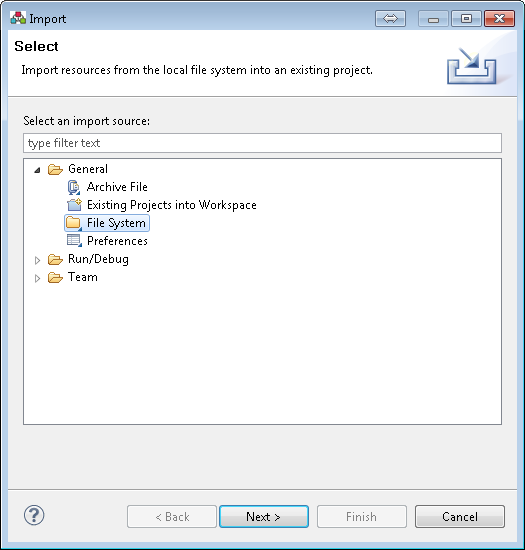
\includegraphics[width=.6\textwidth]{images/DestecsImportDialogFileSystem.png}
%% \caption{Import files into the Crescendo tool.}
%% \end{figure}

%% \begin{figure}[htbp]
%% \centering
%% 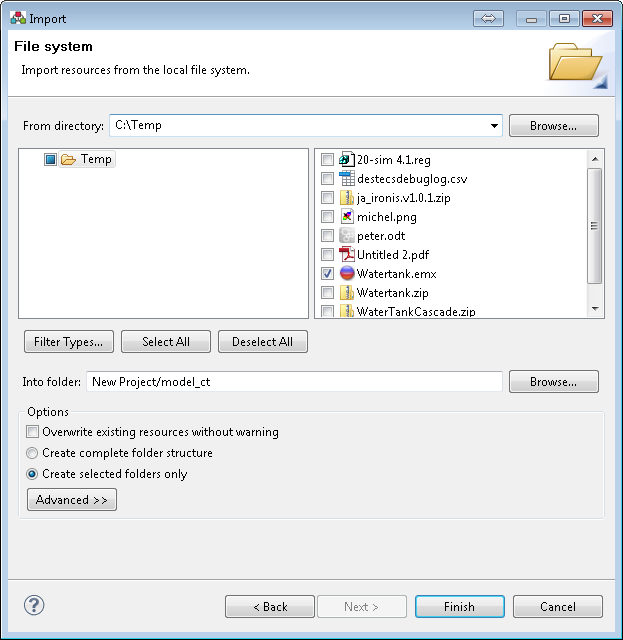
\includegraphics[width=.6\textwidth]{images/DestecsImport20simModel.png}
%% \caption{Choose the file to import.}
%% \end{figure}

%% \begin{itemize}
%% \item
%%   Select the \textbf{20-sim model} from the list of files.
%% \item
%%   Click \textbf{Finish}.
%% \end{itemize}

%% \subsection{Discrete-event Model}

%% \begin{itemize}
%% \item
%%   Select the item~\textbf{model\_de}
%% \end{itemize}

%% \begin{itemize}
%% \item
%%   Right-click and select \textbf{Import} - \textbf{File System.~}
%% \end{itemize}

%% From the \textbf{Import Dialog}, choose \textbf{the~}directory
%% \emph{'that contains the \textbf{VDM~}model}'.

%% \begin{figure}[htbp]
%% \centering
%% 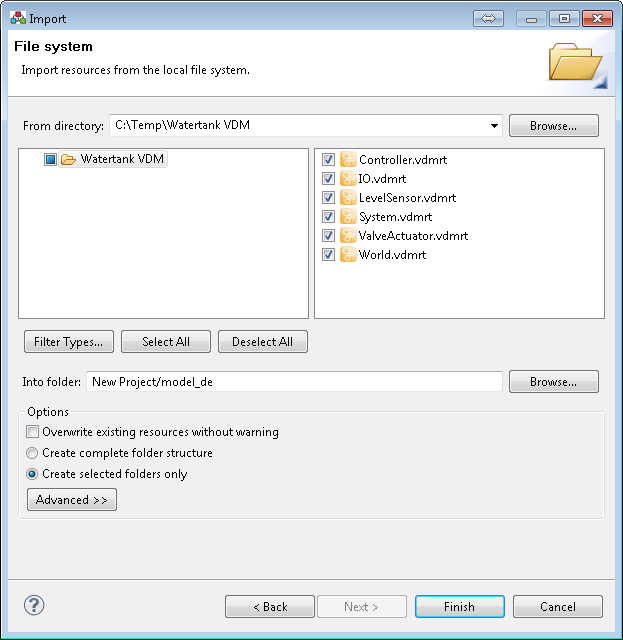
\includegraphics[width=.6\textwidth]{images/DestecsImportVDMmodel.png}
%% \caption{Choose the file to import.}
%% \end{figure}

%% \begin{itemize}
%% \item
%%   Select the directories that comprise the \textbf{VDM~model}.
%% \item
%%   Click \textbf{Finish}
%% \end{itemize}

\section{Managing Contracts}\label{sec:contract}

To connect the Continuous-Time model and Discrete-Event model 
we have to define a \emph{contract}. The contract also needs to be linked
into DE and CT elements respectively.
In order to show the co-simulation tool how to link the elements from
the contract to the DE and CT models respectively a link-file must be
present for each co-model. This is stored in a \emph{vdm.link} part.

\subsection{Creating a new Contract File}

Right click on the project that is going to contain the contract file.
Select \emph{New} and \emph{Crescendo New Contract} as shown in Figure~\ref{fig:newcontract}.

\begin{figure}[htbp]
\centering
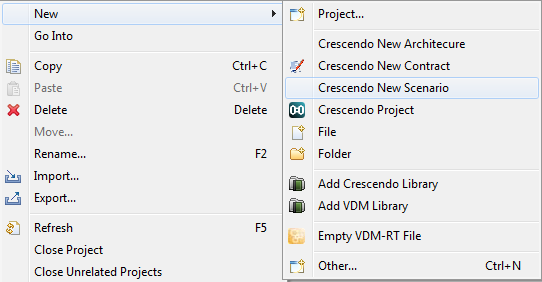
\includegraphics[width=.6\textwidth]{images/DestecsNewContract.png}
\caption{Choosing a new Crescendo contract.\label{fig:newcontract}}
\end{figure}

\begin{itemize}
\item
  A new window will pop up. Choose a \texttt{contract name} and click on
  the \emph{Finish} button to end the process.
\end{itemize}

After following these steps a new file named \texttt{contract.csc} will
appear under the \texttt{con\-fig\-ura\-tion} folder contained in the project
tree. The contract can be viewed in the editor as shown in Figure~\ref{fig:editorcontract2}.

\begin{figure}[htbp]
\centering
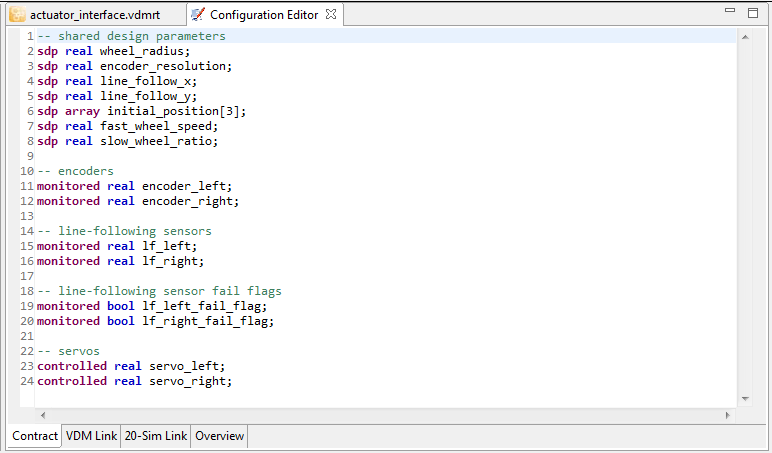
\includegraphics[width=.6\textwidth]{images/DestecsEditorNewContract.png}
\caption{The Editor with a new contract.\label{fig:editorcontract2}}
\end{figure}

\subsection{Contents of a Contract}

A contract between a CT and a DE model can contain the following kind of
information:

\begin{description}
\item[Design parameters:] These are typically values which indicate
  the properties of components (e.g. size, weight, temperature). A
  designer would like to explore different values of these parameters in
  order to find an optimal solution to the challenge he is working on.
  The actual values for the shared design parameters are set outside the
  contract in a separate file.
\item[Variables:] The variables are the active interface between the
  CT and DE models so these indicate the variables that change during
  one simulation. Variables typically represent sensor readings and
  signals to actuators.
\item[Events:] Events can be triggered in the CT world. They
  will stop the simulation before the allowed time slice is completed.
  The co-simulation engine will then allow the DE simulator to
  take~action but only until the point where the event has been raised.
  The events are used in the contract in order to support event-based
  triggering and not just time-triggered scheduling.
\end{description}

The syntax for contracts follow the following rules:

\begin{grammar}
<contract> ::= parameters | variables | events;

<parameters> ::= `shared\_design\_parameter' type identifier `;'
             |   `sdp' type identifier `;'

<variables> ::= kind type identifier `;' 
            |   kind `matrix' identifier shape `;'

<shape> ::= `[' `integer' `,' `integer')* `]' 

<events> ::= `event', identifier, `;'

<type> ::= `real' | `bool' ;

<identifier> ::= initial\_letter (following letter)* ;

<kind> ::= `monitored' | `controlled' ;

<value> ::= float | boolean\_literal ;

<boolean literal> ::= `true' | `false' ;
\end{grammar}

In the following listing, an extract from the contract file provided
with the \texttt{Water\-Tank\-Periodic} example is shown.

\begin{dcl}
-- Shared design parameters
sdp real maxlevel;
sdp real minlevel; 

-- Monitored variables (seen from the DE controller)
monitored real level;

-- Controlled variables (seen from the DE controller)
controlled bool valve; 
\end{dcl}

\subsubsection{Matrices}

It is also possible to exchange matrices
between DE and CT models. To be able to do this, a matrix needs to be
declared in the contract. The adopted syntax is similar to 20-sim, where
the shape of the matrix is indicated by a sequence of integers
{[}m$_1$,...,m$_n${]}. For example, to declare
a 2x2 matrix named \texttt{M} which is \vdmkeyw{monitored} the following must be
added to the contract:

\begin{dcl}
monitored matrix M[2,2];
\end{dcl}

In VDM matrices of ``n'' dimensions
\texttt{(m1 *... * mn)} are
represented as (\vdmkeyw{seq of ... seq of real}). So a 2x2 matrix is
represented as a (\vdmkeyw{seq of seq of
real}).

The contract matrix variables are linked in the same manner as any other
variable but the target variable needs to be of the correct type, in our
case~\vdmkeyw{seq of seq of real}. At the VDM level this would typically 
be declared as:

\begin{vdmrt}
instance variables

    M: seq of seq of real := [[0.0,0.0],[0.0,0.0]];
\end{vdmrt}

\subsubsection{Arrays}

Arrays which are limited to one dimension can be declared in the same style: 

\begin{dcl}
monitored array position[3];
\end{dcl}



\subsection{Error Detection in the Contract/Link File}

A static error check is performed every time the contract or the
link file are saved. This is a
cross-file consistency check which resolves if all the variables/events
declared in a contract are also present in the link and vice-versa.
Crescendo will prevent the launch of projects with consistency errors
between the contract and link files but there is the possibility to turn
this protection off by un-checking the referent preference (accessible
in the menu ``\emph{Windows} followed by \emph{Preferences}''). This is illustrated in Figure~\ref{fig:linkerrors}.

\begin{figure}[htbp]
\centering
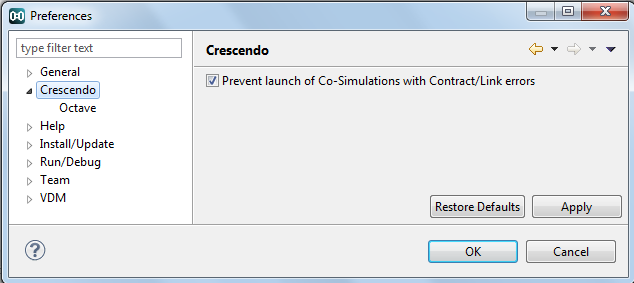
\includegraphics[width=.8\textwidth]{images/DestecsPreferences.png}
\caption{Launching with or without contract or link errors.\label{fig:linkerrors}}
\end{figure}

\subsection{Managing the Link Files}

The link file is automatically created when you start a new project. You
can edit the link file by selecting the configuration folder in the
project tree.

Expand the project and configuration folder and \emph{select the file} \texttt{vdm.link}. Figure~\ref{fig:linkfile} shows the editor with the contents of the link file.


\begin{figure}[htbp]
\centering
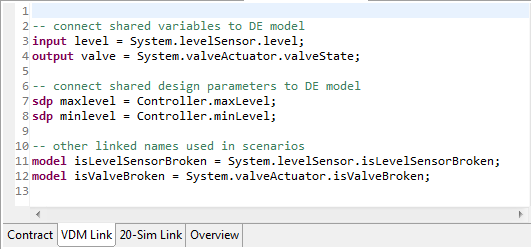
\includegraphics[width=.6\textwidth]{images/DestecsContractFile.png}
\caption{Expand the configuration folder to see the link file.\label{fig:linkfile}}
\end{figure}



\subsubsection{Contents of a link file}

The syntax of a link file is a sequence of link definitions (each
definition is formed by an interface type, a qualified name, ``\texttt{=}'' sign
and a qualified name) separated by line breaks. Here all the design
parameters, the variables and the events from the contract must be
present on the left-hand-side of each of these definitions. It is
important to note that the link file may contain more links than
required by the contract, this allows a DE model to be reused in
different simulations where different contracts are used. Additionally,
links can be made to variables that~exist within the model in order to
be able to reference them from a script (the keyword ``\vdmkeyw{model}'' is used
for this purpose). The right-hand-side of all the ``\texttt{=}'' signs provide
the names seen from the DE co-model side, e.g., the instance variables
inside a system class in the VDM-RT model.

The syntax of these definitions are:

\begin{grammar}
<vdmlink-file> ::= \{ <interface>, <qualified-name>, `=', <qualified-name>, `;' \}

<interface> ::= `output' | `input'  | `sdp' | `event'  | `model'~;

<qualified-name> ::= <identifier>, {[} `.', <identifier> {]}~;

<identifier> ::= <initial-letter>, \{ <following-letter> \}~;
\end{grammar}

\subsubsection{Link File Parts}

\begin{itemize}
\item
  \vdmkeyw{input} links one monitored variable in the contract with a
  instance variable in the DE model. The qualified name must start with
  the system class name.
\item
  \vdmkeyw{output} links one controlled variable in the contract with
  an instance variable in the DE model. The qualified name must start
  with the system class name.
\item
  \vdmkeyw{sdp} links a shared design parameter in the contract with
  a value in the DE model. The qualified name can start by any
  class name and the referenced value must be a ``value'' in VDM.
\item
  \vdmkeyw{model} links a ``name'' and a variable in the VDM model. The
  name can then be used to reference the variable in scripts.~The
  qualified name must start with the system class name.
\end{itemize}

The \texttt{vdm.link} file for the \texttt{WaterTankPeriodic} example looks as:

\begin{dcl}
-- connect shared variables to DE model
input level = System.levelSensor.level; 
output valve = System.valveActuator.valveState;

-- connect shared design parameters to DE model
sdp maxlevel = Controller.maxLevel;
sdp minlevel = Controller.minLevel;
	
-- other linked names used in scenarios
model isLevelSensorBroken = 
                   System.levelSensor.isLevelSensorBroken;
model isValveBroken = 
                   System.valveActuator.isValveBroken;
\end{dcl}

\subsubsection{CT Model}

On the 20-sim side, a link file is not used, but still, the
variables/parameters need to be declared in a certain way inside the 20-sim model in order to
carry out the co-simulation.

%%\subsection{Co-simulation variables}

Variables used in the co-simulation, need to be in the
\vdmkeyw{externals} field and marked as \vdmkeyw{global}. Depending if
they are used as input or output they need to be marked
\vdmkeyw{import} or \vdmkeyw{export} respectively. Example:

\begin{dcl}
externals
  real global export level;
  real global import valve;
\end{dcl}

%%\subsection{Shared Design Parameters}

The parameters to be shared across the two models need to be marked with
the keyword \vdmkeyw{shared}. Example:

\begin{dcl}
parameters
  real aParam ('shared') = 5; 
\end{dcl}

%%\subsection{Events}

Events need to be marked using the \vdmkeyw{event} keyword this marks
the variable that it used as return value of the event function to be an
event variable.~The keywords \vdmkeyw{eventdown} and \vdmkeyw{eventup}
are used as in standalone 20-sim models. Example:

\begin{dcl}
variables
  boolean minLevelReached ('event');
equations
  maxLevelReached = eventup(levelIn-maxlevel);
\end{dcl}

\subsection{Contract Overview}

An overview of the contract can be seen on the last tab of multi-editor as shown in Figure~\ref{fig:ContractOverview}.

\begin{figure}[htbp]
\centering
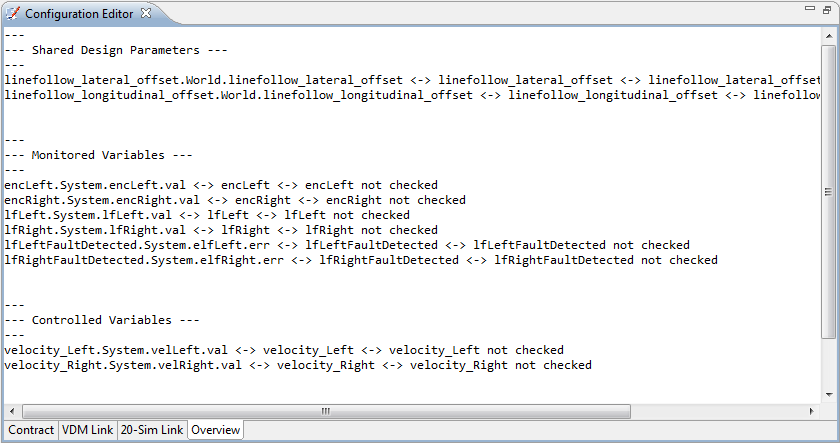
\includegraphics[width=.8\textwidth]{images/ContractOverview.png}
\caption{Overview of contract information.\label{fig:ContractOverview}}
\end{figure}

In this view it is possible to see which variable from the DE side is
connected to which contract variable and transitively to which CT
variable. The form they are presented is:

\begin{verbatim}
VDM variable <-> Contract Variable <-> 20-sim variable
\end{verbatim}

The ``\emph{not checked}'' appears next to the 20-sim variables because at
this moment is not possible to static check if the variables exist in
the 20-sim model.


\chapter{Co-Simulation Possibilities}\label{chap:cosim}

\section{Debug Configuration}\label{sec:DebugConfigIntro}

Before starting a co-simulation, a debug configuration must be created
if a launch configuration is not already available.
The purpose of this is to define where the Continuous Time and Discrete
Event models are located, as well as the scenario file and the
simulation time. In this section we will go through each pane in the debug configuration.

\subsection{Creating a New Debug Configuration}

\begin{itemize}
\item
  \emph{Select the project} for which you want to create a Debug
  Configuration.
\item
  Press the \textbf{small arrow} next to the debug icon
  
\includegraphics{images/DestecsDebugButtonArrow.png}~at the top of the
  the Crescendo Tool.
\item
  A drop-down menu will appear, in which the option
  \emph{Debug configuration} has to be selected, and as a consequence
a new window as shown in Figure~\ref{fig:DestecsDebugConfigurationNew}.
\item
  Select the option \emph{Co-Sim Launch} and
  \emph{New Configuration}
\end{itemize}

\begin{figure}[htbp]
\centering
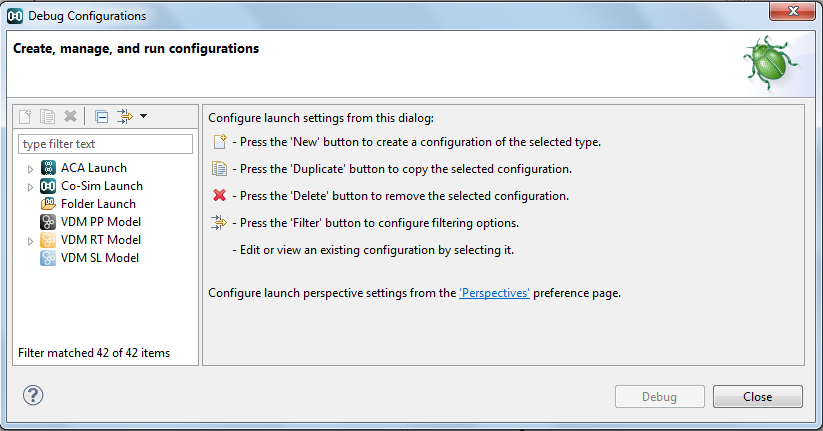
\includegraphics[width=.6\textwidth]{images/DestecsDebugConfigurationNew.png}
\caption{Select a new debug configuration.\label{fig:DestecsDebugConfigurationNew}}
\end{figure}

Now a window will show up as Figure~\ref{fig:DestecsDebugConfigurationMain}
where you can enter the settings of the debug
configuration. We will describe all the tabs that can be configured before running a
co-simulation.

\subsection{Main Tab}

\begin{figure}[htbp]
\centering
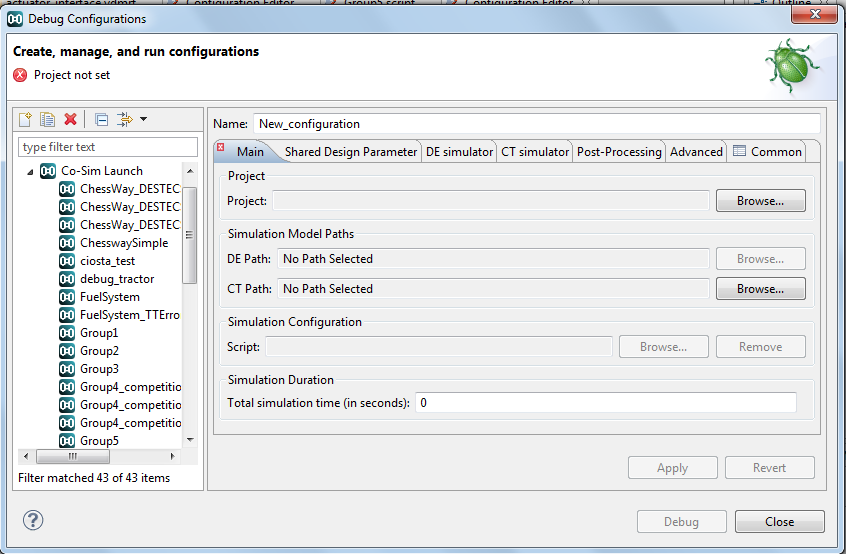
\includegraphics[width=.8\textwidth]{images/DestecsDebugConfigurationMain.png}
\caption{The Main tab of the Debug Configuration.\label{fig:DestecsDebugConfigurationMain}}
\end{figure}

%\begin{itemize}
%\item
%  Click the \emph{Browse} button to \emph{select your project}.
%\end{itemize}

%Once the~project is found and selected, the path for the Discrete-Event model will be automatically set. Since multiple Continuous-Time
%models could be present the \emph{Browse} button to select the one
%you would like to use.
%
%\begin{itemize}
%\item
%  Click on the ``\emph{Browse}'' button to \emph{select the script file}
%  (if a script file is available --- see Section\ref{sec:scenarios} for more information on script files).
%\item
%  Set the option ``\emph{Total simulation time}'' which defines for how 
%  many seconds the simulation is going to take into account.
%\end{itemize}

The Main Tab is where the project to co-simulate is selected. This can
be done by pressing the ``\emph{Browse...}'' button. After selecting the
wanted project, the DE model path is automatically filled
since it is only possible to have one DE model in the \texttt{model\_de}
folder. Though the CT model path needs to be selected using the \emph{Browse...}
button. If a scenario should be used (see Section\ref{sec:scenarios} for more information on scenarios), it is possible
to select which one in the Simulation Configuration section. The total
simulation time should be a number greater than zero to be able to run
the co-simulation.

\subsection{Shared Design Parameters Tab}

An important feature of the debug configuration is the possibility to
view and modify the \emph{shared design
parameters} of the co-simulation. This is configures in Figure~\ref{fig:sdpindebug}. 

\begin{figure}[htbp]
\centering
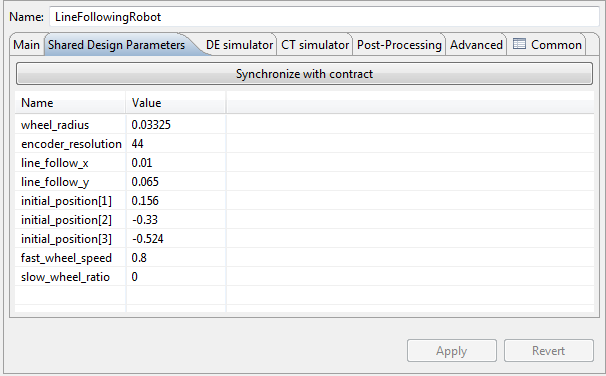
\includegraphics[width=.6\textwidth]{images/DestecsDebugConfigurationSDP.png}
\caption{The Shared Design Parameters tab of the Debug Configuration.\label{fig:sdpindebug}}
\end{figure}

%\begin{itemize}
%\item
%  Click \emph{Synchronize with contract} to import the shared design
%  parameters.
%\item
%  \textbf{Set the parameters} to their proper values.
%\end{itemize}

In the \emph{Shared Design Parameters} tab, a list of the parameters used in
the simulation can be viewed. For the variables to appear for the first
time the the button ``\emph{Synchronize with contract}'' needs to be pressed.
Every time the shared design parameters are changed in the contract, the
button must be pressed again in order to synchronize the view with the
contract.

For the variables present in the table
it is possible to decide which values they will have when the
co-simulation starts. Figure~\ref{fig:sdpindebug} shows the Shared Design
Parameters tab for a project that has an array[3] as a shared design
parameter.

\subsection{DE Simulator Tab}

The \emph{DE Simulator} tab is the tab where runtime options for the DE part of
the model can be activated/deactivated. It is divided in 4 options
groups:

\begin{description}
\item[Interpreting:] These are options related with the interpretation of
  the DE models. Certain checks and also the generation of reports such
  as coverage or the real-time events can be turned on/off. Usage of these
  options are further explained in the Overture/VDM user manual \cite{Larsen&13a}.
\item[Log:] In this group it is possible to select variables from the DE
  model that should be logged during the simulation. To find more
  details about this feature, see Section~\ref{sec:Logfiles}.
\item[Faults:] In this group it is possible to
  chose a class \texttt{A} to replace a class \texttt{B} before the co-simulation start. The
  intention is to experiment with faulty modules that can be substituted
  by the non-faulty model. To make sure there will be no run-time
  exceptions, class \texttt{B} should be subclass of \texttt{A}. To indicate that class \texttt{A}
  should be substituted by class \texttt{B}, the following should be inserted in
  the text box \emph{DE Replace Pattern (A/B)}. It is possible to make several
  substitutions by separating the substitutions with a comma
  \texttt{A/B,C/D,...}.
\item[Architecture:] In this area it is
  possible to select an architecture file that defines the architecture
  of the deployment of the DE controller. More information on the
  architecture file can be seen in Section~\ref{sec:DEArch}.
\end{description}

\begin{figure}[htbp]
\centering
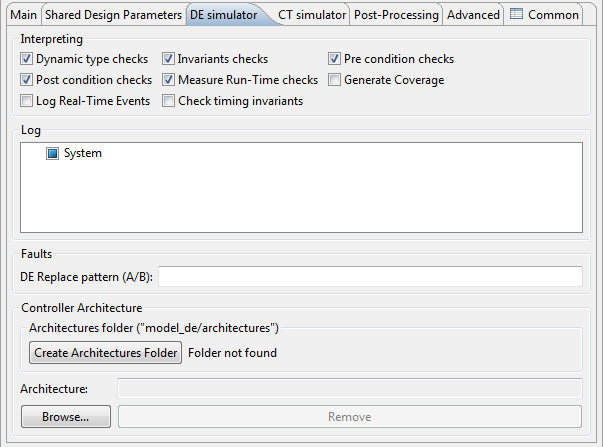
\includegraphics[width=.6\textwidth]{images/DestecsDebugConfigurationDESimulator.png}
\caption{The DE simulator tab of the Debug Configuration.}
\end{figure}

\subsection{CT Simulator Tab}

The 20-sim Options tab contains options related with the execution of
the CT model. At first, both tables (Log and Settings) contain only the
previously saved settings, if no settings were previously selected then
the tables will be empty; the tables can be populated by pressing the
"\emph{Populate...}" button. The "\emph{Populate..}."~button launches
the model selected in 20-sim model and dynamically extracts the settings
and the variables present in the model. As shown in Figure~\ref{fig:CTSimInDebug} there is two areas present
in the 20-sim options tab:

\begin{description}
\item[Log:] In this area it is possible to select which CT variables
  should be logged during the co-simulation execution.
\item[Settings:] The settings are presented in a tree view. In this tree
  there is two types of nodes, option nodes and ``virtual'' nodes which
  are only there to give the tree structure. If an option node is
  selected, the different possibilities will be presented on the right
  side (``\emph{Options}'' group).
\end{description}


\begin{figure}[htbp]
\centering
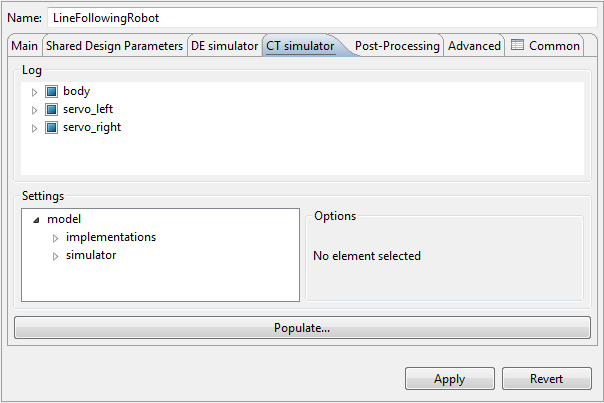
\includegraphics[width=.6\textwidth]{images/DestecsDebugConfigurationCTSimulator.png}
\caption{The CT simulator tab of the Debug Configuration.\label{fig:CTSimInDebug}}
\end{figure}


\section{Post-Processing Tab}

The post processing tab shows the options available for the
post-processing phase (see Figure~\ref{fig:postproctab}).

\begin{figure}[htbp]
\centering
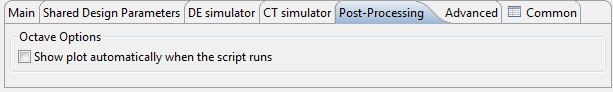
\includegraphics[width=.6\textwidth]{images/Postprocessingtab.png}
\caption{Post-processing tab for debug configuration.\label{fig:postproctab}}
\end{figure}

``Show plot automatically when the script runs'' with this option
enabled, the Octave script that is generated after each run will
contain the commands to show the plot automatically, i.e., simply
running the script will show the plots. For more information on the use of Octave, please see Section~\ref{sec:octave}.

\subsection{Advanced Tab}

The advanced tab is reserved for developers, extra debug information can
be turned on or off in this tab (see Figure~\ref{fig:advancedtab}). 
%More detail on the extra debug
%information can be found in \href{Debug_Reports}{Debug Reports}

\begin{figure}[htbp]
\centering
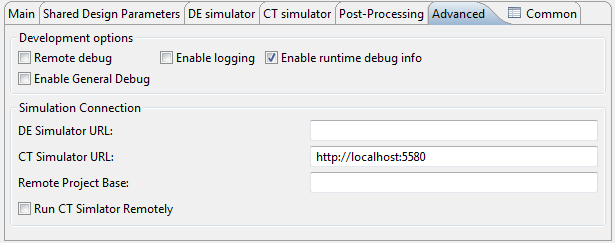
\includegraphics[width=.6\textwidth]{images/Advancedoptionstab.png}
\caption{Advanced options tab.\label{fig:advancedtab}}
\end{figure}

\subsection{Common Tab}

The Common tab is a standard Eclipse tab which, for example, allows
users to save the debug configurations into files so that they can be
shared with others. Figure~\ref{fig:commontab} shows how to produce a launch file that can be shared with others.

\begin{figure}[htbp]
\centering
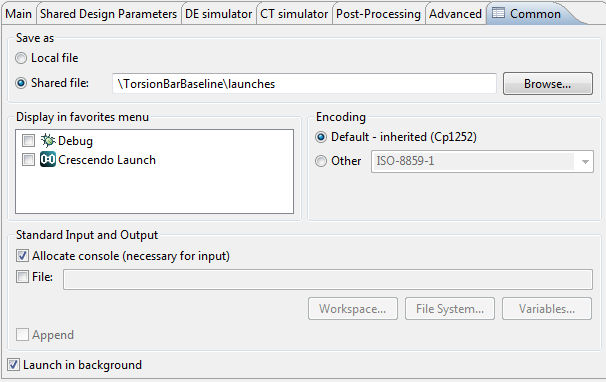
\includegraphics[width=.6\textwidth]{images/Commontab.png}
\caption{This is where launch files can be created.\label{fig:commontab}}
\end{figure}

\section{Scenarios}\label{sec:scenarios}

%%\subsection{Introduction}

%% Current version of Crescendo tool supports two different kinds of syntaxes
%% for the script languages:

%% \begin{enumerate}
%% \item
%%   \textbf{with the extension name ".script"}: For each project it is
%%   possible to define a large collection of scenarios. From a
%%   discrete~event perspective, these scenarios can be thought off as test
%%   cases. Each scenario can be considered as a sequence of external
%%   stimuli to the co-simulation. Each stimulus has a time associated with
%%   it (that is when the stimuli is injected into the simulation). In
%%   addition each stimulus has an action associated with it. Such actions
%%   can set variables either at the CT or the DE side of the simulation. ~
%% \item
%%  \textbf{with the extension name ".script2"}: this 
Scripts allow users
  to define condition-action pairs (using a statement called
  \texttt{\textbf{when}}), which perform an action \emph{when} the condition becomes true during
  a co-simulation. This script allows these conditions to reference the
  current co-simulation time and the state of the co-model, and to
  combine them with logical operators. Actions can make assignments to selected
  parts of the co-model and also provide information back to the user,
  as well as terminating the simulation.
%%\end{enumerate}

This section describes how to create scenario files and introduces
a command language for Crescendo scripts called CSL (Crescendo
Scripting Language). The main purpose of CSL is to allow engineers to
simulate user input and activate latent non-normative behaviours during
a co-simulation. The language is designed to be~sufficiently rich as to
allow engineers to influence a co-model during co-simulation, without
being overly complex. For example, it does not allow local variables to
be defined.

\subsection{Creating a New Scenario File}

Follow these steps in order to create a new scenario file:

\begin{itemize}
\item
  Right-click on the project that is going to contain the contract file.
  Select ``\emph{New}'' and \emph{Crescendo New Scenario}.
\item
  A new window will pop up, named \emph{Scenario Wizard}. Select the
  current project by clicking on the ``\emph{Browse}'' button. Click on the
  \emph{Finish} button to end the process.
\end{itemize}

After following these steps a new file named \emph{Scenario.script2}~will
be placed under the scenarios folder. 
%To use the \texttt{script2} functionality
%the extension of script file needs to be changed to ``script2''.

%\subsection{Scripts with extension name ".script"}

%The syntax of each scenario file needs to be:

\subsection{CSL Syntax}

Here we give the syntax of the CSL using standard notation.  Note that
the definitions of \synt{real-literal}, \synt{name}, and \synt{string}
are not given.

\begin{grammar}
<script> ::= <trigger> <script> | <trigger>

<trigger> ::= <trigger-type> <expression> <duration> `do' <body> <after>

<trigger-type> ::= `when' | `once'

<expression> ::= `time' | <literal> | <identifier> | <unary-expression> | <binary-expresion>

<literal> ::= <boolean-literal> | <real-literal>

<boolean-literal> ::= `true' | `false'

<identifier> ::= <simulator> <type> <name>

<simulator> ::= `de' | `ct'

<type> ::= `boolean' | `real'

<unary-expression> ::= <unary-operator> <expression>

<unary-operator> ::= `not' | `+' | `-' | `abs' | `floor' | `ceil'

<binary-expression> ::= <expression> <binary-operator> <expression>

<binary-operator> ::= `+' | `-' | `*' | `/' | `**' | `div' | `mod' | `<' | `<=' | `=' | `>=' | `>' | `<>' \\| `and' | `or' | `=>' | `<=>'

<duration> ::= <empty> | `for' <real-literal> `{' <time-unit> `}'

<time-unit> ::= `us' | `ms' | `s' | `m' | `h'

<body> ::= <block> | <statement>

<block> ::= `(' <statement-list> `)'

<statement-list> ::= <statement> | <statement> `;' <statement-list>

<statement> ::= <identifier> `:=' <expression>
 \alt `print' <string>
 \alt `warn' <string>
 \alt `error' <string>
 \alt `quit'

<after> ::= `after' <revert-list>

<revert-list> ::= `revert' <identifier> | `revert' <identifier> `;' <revert-list>
\end{grammar}

%\subsection{CSL Examples}
%
%\begin{dcl}
%when time > 60 {s} do
%  print "Past one minute"
%\end{dcl}
%
%\begin{dcl}
%when de boolean active = true for 2 {m} do
%  ( print "Controller active for two minutes" ;
%    de boolean sensor = false )
%after
%  revert de boolean sensor
%\end{dcl}

%% scenario file = \{ numeric literal, (`\textbf{DE}' \textbar{}
%% `\textbf{CT}'), `.', identifier, `:=', symbolic literal \}, `;'~;

%% identifier = initial letter, \{ following letter \}~;

%% symbolic literal = numeric literal \textbar{} boolean literal
%% \textbar{}~nil literal \textbar{} character literal \textbar{} text
%% literal \textbar{}~quote literal~;\\boolean literal = `\textbf{true}'
%% \textbar{} `\textbf{false}'~;

%% text literal = ` " ', \{ ` \textbackslash{}" ' \textbar{} character
%% \textbar{} escape sequence \}, ` " '~;

%% quote literal = `\textless{}', identifier, `\textgreater{}'~;

%% In the following listing, an extract from the scenario file provided
%% with the water tank introductory example is shown.

%% \begin{dcl}
%% 2.5 DE.fault := 2.33;
%% 1.0 CT.Control\testSignal=1
%% \end{dcl}

%% Essentially the meaning of a scenario is simply that the indicated
%% changes of the variables either~on the DE or the CT side is changing at
%% the time (the first value in all cases) to the value provided~after the
%% \texttt{:=} sign. So these can be considered as disturbances provided for the
%% simulation at~the specific time and thus each such a file correspond to
%% one scenario. Sweeping over for example~different design parameters will
%% be done with a kind of higher level scenario as a part of the
%% Design~Space Exploration feature to be developed as a part of the
%% Crescendo tool suite.~


%% We assume that \textbf{digit}, string, and file path have their obvious
%% definitions. Since no variables can be defined in the script language,
%% all identifiers will exist in the co-model and therefore identifier
%% literal will conform to the conventions of VDM and 20-sim.

\subsection{CSL Examples}

The following introduces a series of simple examples that demonstrate
the features of this script language.

\begin{dcl}
when time = 5 do

(de real x := 10;);
\end{dcl}

The \vdmkeyw{time} keyword yields the current co-simulation time. The \vdmkeyw{de}
keyword indicates that \texttt{x} resides (at the top level) in the DE
model. Naturally, the \vdmkeyw{ct} keyword is used to indicate the CT model.
Comments may also be included:

\begin{dcl}
when time = 5 do
// comment
(ct real y := true;);
\end{dcl}

Statements can also be grouped in blocks (surrounded by parentheses and
separated by semicolons. Expressions of time can optionally include a
unit (e.g.\ milliseconds) given in curly braces. Units are assumed to be
in seconds if no unit is given. The engineer may output messages to the
tool (or to a log in batch mode) with the \vdmkeyw{print} statement:

\begin{dcl}
when time = 900 {ms} do
(
de real x := 10;
ct real y := true;
print "Co-simulation time reached 900 ms.";
);
\end{dcl}

Logical operators can be used in expressions. When the condition becomes
true, the statement(s) in the do clause will execute. 

\begin{dcl}
when time >= 10 and time < 15 do
(print "Co-simulation time reached 10 seconds.";)
\end{dcl}

If the condition
becomes false again, the optional \texttt{\textbf{after}} clause will execute once. Note
that block statements do not permit local variables to be defined. Since this script language does not allow local variables to be defined,
a special statement, \texttt{\textbf{revert}}, may be used in an \texttt{\textbf{after}} clause to change a
value back to what it was when the do clause executed.

\begin{dcl}
when time >= 10 and time < 15 do 
(// assume x = 5
 de real x := 10;
)
after (revert de real x;);
\end{dcl}

The engineer can reference co-model state in conditions and assignment
and revert statements. The state that can be referred is either for VDM
specified with the \vdmkeyw{model} keyword in the link file or for 20-sim
marked as global (note 20-sim access is not yet implemented).
Additionally all shared variables can be accessed with the contract name
and used in conditions, assignments or revert statements.

It is also possible to have some statements executed exactly once, on
the first time a condition is detected. This is acheived using the
\vdmkeyw{once} keyword instead of \vdmkeyw{when}.

\begin{dcl}
once de real x >= 500 do
(
// set some flag
de bool flag = true;
print "First time x exceeds 500";
)
\end{dcl}

\section{Logfiles}\label{sec:Logfiles}

When starting a simulation, it is possible to select a set of variables
that are logged throughout the co-simulation. At the moment of writing this manual
there is only the possibility of logging DE variables;
support to log CT variables will be added later. The result of this
logging is a CSV file (comma separated values).

\subsection{DE Variables}

The variables of the DE model to log can be selected in the tab VDM
Options presented in Figure~\ref{fig:logvariables}. If a model does not contain type
errors, this tab will display all instance variables that are accessible
from the VDM \vdmkeyw{system} class.

\begin{figure}[htbp]
\centering
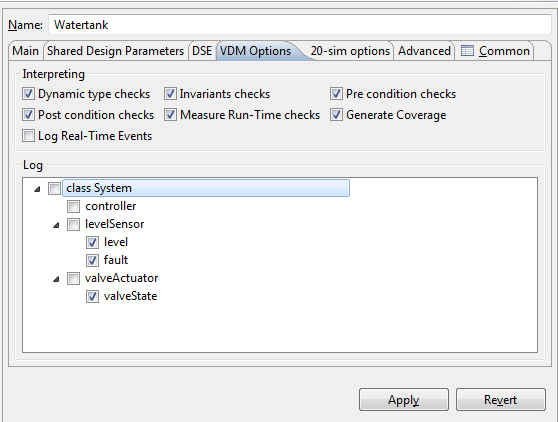
\includegraphics[width=.6\textwidth]{images/Destecsloggingvariables.PNG}
\caption{VDM Options tab permits the selection of variables to log.}
\label{fig:logvariables}
\end{figure}

Checking the box next to a variable enables the logging of that
variable. Currently it is only possible to log variables with basic
types (all types except objects).

For the \texttt{WatertankPeriodic} example, if we use the configuration
shown above, a file with the contents as follows is generated:

\begin{verbatim}
time_,levelSensor.fault,levelSensor.level,valveActuator.valveState

0.0,0,0,0

0.01,0,0.01,0

0.01,0,0.02,0

0.02,0,0.03,0

0.03,0,0.03,0

... ... ... ...
\end{verbatim}

The first column is the time and the following ones are the value of the
variable at the given moment. A CSV file can be better visualized, for
example, in \emph{20-sim}, \emph{Excel} or other software capable of
opening this format.

%% \section{Debug Reports}

%% Once the simulation has been completed, a set of log files will be
%% generated. The contents of~these files are displayed while the
%% simulation is running in the \href{Overview}{simulation logging views}.
%% Even though those records are shown on the tool, it might be useful to
%% have them~logged to external files for further post-simulation analysis.

%% \subsection{The Engine.log File}

%% The Engine.log file is registering the events indicated from the
%% discrete event simulation, noted by \emph{VDM-RT} in the beginning of
%% the entry, from the continuous simulation (indicated by \emph{20-sim} in
%% the beginning of the entry) or both (labelled \emph{All}). As an example
%% of an \emph{Engine log}, an extract from the one generated after the
%% WaterTank simulation is shown below.

%% As it can be seen, it is registered how the engine has been loaded,
%% which design parameters are going to be used and the versions
%% corresponding to the different continuous time and discrete event
%% simulation applications. Paths to the exact models and the loading
%% actions together with their results are monitored as well.

%% \begin{verbatim}
%% All , Simulation engine type loaded:
%% org.destecs.core.simulationengine.ScenarioSimulationEngine
%% All , Shared Design Parameter initialized as:
%% (maxlevel:=0.0 minlevel:=0.0 )
%% VDM-RT , Launching
%% VDM-RT , Interface Version: name: VDMJ version: 0.0.0.1
%% VDM-RT , Initilized ok: true
%% 20-Sim , Interface Version: name: 20-sim version: 4.1.2.3
%% 20-Sim , Initilized ok: true
%% VDM-RT , Loading model:
%% C:\Users\ja\DestecsIde-0.0.2\workspace\watertank_new\model
%% VDM-RT , Loading model completed with no errors: true
%% 20-Sim , Loading model:
%% C:\Users\ja\DestecsIde-0.0.2\workspace\watertank_new\
%% watertank_new.emx
%% 20-Sim , Loading model completed with no errors: true
%% VDM-RT , Interface =&gt; Design P( maxlevel minlevel )
%% Inputs( level ) Outputs( valve )
%% 20-Sim , Interface =&gt; Design P( Control\maxlevel
%% Control\minlevel Control\testSignal )
%% Inputs( valve ) Outputs( level )
%% All , Validating interfaces...
%% All , Validating interfaces...completed
%% \end{verbatim}

%% Once simulation time is over, the engine will send termination commands
%% to each continuous and~discrete simulations. This is notified in a three
%% stepped way, indicating that the process is going~to be terminated,
%% indicating that the process has been sent the kill command and finally a
%% done~message. As it can be seen, the labels \emph{VDM-RT} and
%% \emph{20-sim} are used to indicate whether the~message is referring to
%% the continuous time or the discrete event simulation.

%% \begin{verbatim}
%% VDM-RT , Terminating...
%% VDM-RT , Terminating...kill
%% VDM-RT , Terminating...done
%% 20-Sim , Terminating...
%% 20-Sim , Terminating...kill
%% 20-Sim , Terminating...done
%% \end{verbatim}

%% \subsection{The Message.log File}

%% The \emph{Message.log} file is logging the the messages coming from both
%% \emph{VDM-RT} discrete and\emph{20-sim} continuous simulation. In the
%% following listing, the contents of the ''Message.log ''file for
%% the~water tank example are shown. Note that that the structure this file
%% is presenting is similar to the~co-simulations run by the Crescendo tool.
%% As it can be seen, the first step is to check the version~of the
%% components so they can be initialized and loaded afterwards. The next
%% step is to query the~interface for the simulation engine and set the
%% appropriate design parameters. Once those preliminary actions have been
%% executed the simulation can be started.

%% \begin{verbatim}
%% VDM-RT , getVersion , 0.0
%% VDM-RT , initialize , 0.0
%% 20-Sim , getVersion , 0.0
%% 20-Sim , initialize , 0.0
%% VDM-RT , load , 0.0
%% 20-Sim , load , 0.0
%% VDM-RT , queryInterface , 0.0
%% 20-Sim , queryInterface , 0.0
%% VDM-RT , setDesignParameters , 0.0
%% VDM-RT , start , 0.0
%% 20-Sim , start , 0.0
%% VDM-RT , step , 0.0
%% \end{verbatim}

%% As in the case of the Engine.log file the terminating signals are
%% registered as well in the~Message.log file. See the listing below.

%% \begin{verbatim}
%% VDM-RT , stop , 10.0
%% VDM-RT , terminate , 10.0
%% 20-Sim , terminate , 10.0
%% \end{verbatim}

%% \subsection{The Simulation.log File}

%% The \emph{Simulation.log} file is reflecting the evolution of the
%% different parameters under study~in a given co-simulation. In the
%% \url{WaterTank} example this is focused on the values of the
%% variables~''level ''and \emph{valve} and thus these are logged (see
%% listing below).

%% \begin{verbatim}
%% VDM-RT , valve=0.0 , 2.0
%% 20-Sim , level=2.0 , 2.0
%% VDM-RT , valve=0.0 , 4.0
%% 20-Sim , level=4.0 , 4.0
%% VDM-RT , valve=0.0 , 6.0
%% 20-Sim , level=6.0 , 6.0
%% VDM-RT , valve=0.0 , 8.0
%% 20-Sim , level=8.0 , 8.0
%% VDM-RT , valve=0.0 , 10.0
%% \end{verbatim}

%% This is definitely a valuable collection of data, since it can be
%% exported as data files for analysis by~external tools.

\chapter{Design Space Exploration Posibilities}\label{chap:DSE}

In order to support Design Space Exploration (DSE), the Automated
Co-model Analysis (ACA) feature enables automatically running many different
co-simulations with minimal user intervention. The ACA feature enables
the user to select different configurations for each individual parts of
the co-model and then runs the co-simulation combining all possible
configurations that were selected by the user.

\section{ACA Workflow}

Figure~\ref{fig:acaworkflow} illustrates the steps in the process of the ACA work
flow. First the user provides configurations for different parts of the
co-simulation, then the tool generates different complete configurations
by combining the different configurations parts that were provided by
the user.

\begin{figure}[htbp]
\centering
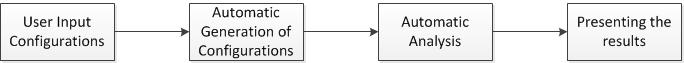
\includegraphics[width=.6\textwidth]{images/ACAworkflow.jpg}
\caption{Illustration of the ACA process.}
\label{fig:acaworkflow}
\end{figure}

These complete configurations are used to execute co-simulations. 
Currently, it is only possible for the user to select different
configurations for different parts of the co-simulation, more
specifically, chose different architectures for deployment of the
controller (DE side), and select different starting values for the
shared design parameters.

\begin{figure}[htbp]
\centering
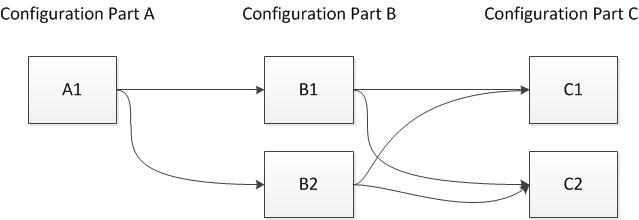
\includegraphics[width=.6\textwidth]{images/ACAconcept.jpg}
\caption{Illustration of the ACA process.}
\label{fig:acaprocess}
\end{figure}

From these partial configurations it is possible to construct complete
configurations by combining each of the different partial
configurations. Figure~\ref{fig:acaprocess} together with the following description
helps illustrating the concept. The result of generating complete
configurations from the partial configuration would be 4 different
complete configurations: A1-B1-C1; A1-B1-C2; A1-B2-C1; and A1-B2-C2. The
user can easily get many more configurations by adding more parameters
or adding more values to existing parameters, for example, simply adding
a A2 value would result in 4 more different configurations.

\section{Using the ACA Features}

Launching an ACA is done through the Debug Configuration menu.
%% \begin{figure}[htbp]
%% \centering
%% 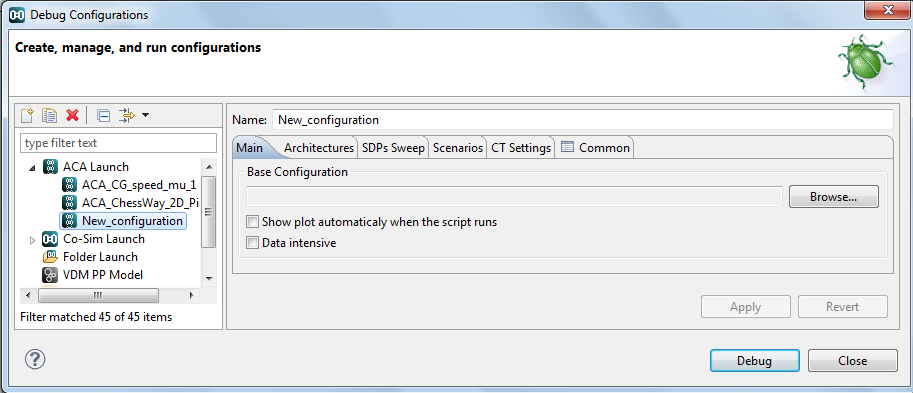
\includegraphics[width=.6\textwidth]{images/DestecsACAdebugconfig.png}
%% \caption{ACA Launch in the Debug Configuration Menu.}
%% \end{figure}
Creating a new Debug Configuration of an ACA Launch type will bring up
the menu to configure the ACA. The different tabs in Figure~\ref{fig:acadebugconfig}, will be explained in the following subsections.

%the several present tabs (The rightmost tab, the Common
%tab, will not be mention here since is a standard Eclipse tab) will be
%explained~individually in the following subsections.

\begin{figure}[htbp]
\centering
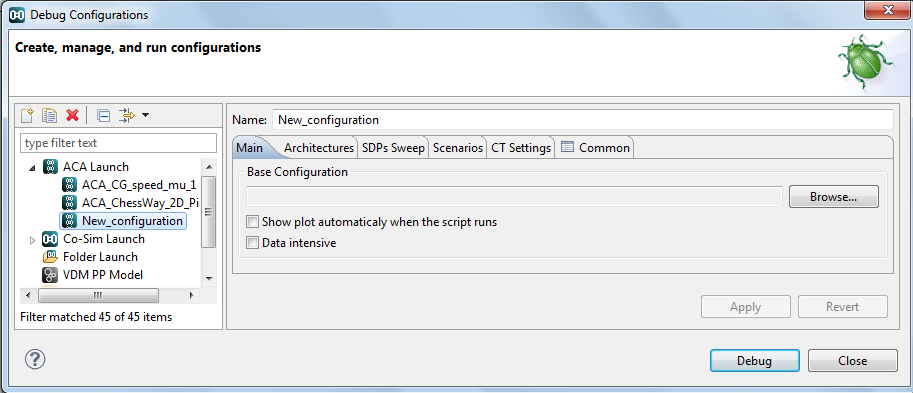
\includegraphics[width=.6\textwidth]{images/DestecsACAdebugconfig.PNG}
\caption{}
\label{fig:acadebugconfig}
\end{figure}

To start an ACA launch, a base configuration needs to be selected. This
configuration is a normal Crescendo launch which will be used as base for
the ACA settings. This means that launch options that are not
overwritten in the ACA will use as default the ones present in the base
launch.

\subsection{The Main Tab}

The Main tab is the place where general settings for the ACA launch
are set. Here the Base Configuration first of all needs to be selected.
The Base Configuration is the co-simulation configuration that
forms the base for the ACA to work. In addition there are two choices that can
be made as shown in Figure~\ref{fig:Destecsacamaintab}. 
%These are:

\begin{itemize}
\item The first option allows the model designer to use the usual plots shown at the 20-sim side for each single co-simulation or to not spending time on that.
\item The second option can be ticked if a huge amount of data is expected to be produced. If this is ticked the data generated are not included in the directory used by the Crescendo tool (in general Eclipse does not like to have a very high number of files). 
\end{itemize}

\begin{figure}[htbp]
\centering
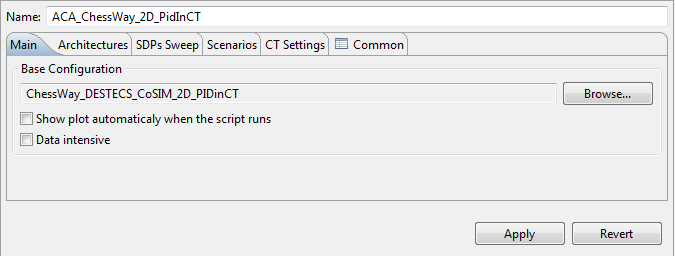
\includegraphics[width=.6\textwidth]{images/Destecsacamaintab.png}
\caption{ACA Launch - Main tab.\label{fig:Destecsacamaintab}}
\end{figure}

By pressing the button Browse it is
possible to browse through the Co-Sim Launches present in the Crescendo
Tool and chose one. This configuration will be the base configuration
for all the ones generated by the ACA. The ACA will take the base
configuration and combine it in all possible ways depending on what the
user set on the other tabs.

\subsection{The Architecture Tab - Deployment Architectures}

In this tab it is possible to select which Controller Architectures will
be used in the ACA run (see Figure~\ref{fig:ArchitecturesACA}. For more information on Controller Architectures
and how to define them please see Section~\ref{sec:DEArch}.

\begin{figure}[htbp]
\centering
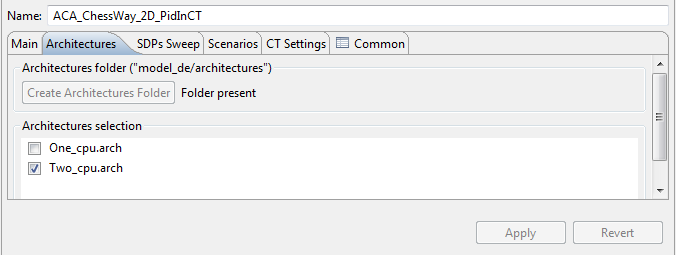
\includegraphics[width=.6\textwidth]{images/ArchitecturesACA.png}
\caption{ACA Launch - Architecture tab.\label{fig:ArchitecturesACA}}
\end{figure}

\subsection{Shared Design Parameters Tab}

In the Shared Design Parameters tab it is possible to make a value
``sweep'' of the shared design parameters (see Figure~\ref{fig:SDPsSweep}).

\begin{figure}[htbp]
\centering
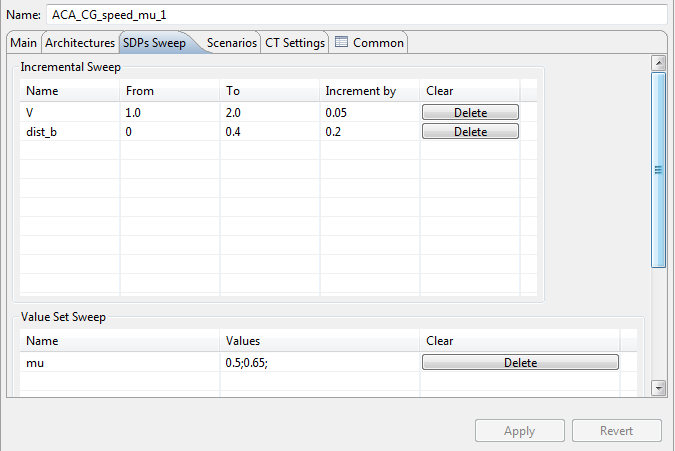
\includegraphics[width=.6\textwidth]{images/SDPsSweep.png}
\caption{ACA Launch -- Shared Design Parameters tab.\label{fig:SDPsSweep}}
\end{figure}

\subsubsection{The incremental Sweep}

In the first column it is possible to select from a drop-down the shared
design parameter to sweep (see Figure~\ref{fig:IncrementalSweep}). 
In the second column (\texttt{From}), it is possible
to select the value which the sweep should start from. The third column
(\texttt{To}) indicates where the sweep should end and the forth column
(\texttt{Increment By}) indicates the increment to be used in the sweep.

\begin{figure}[htbp]
\centering
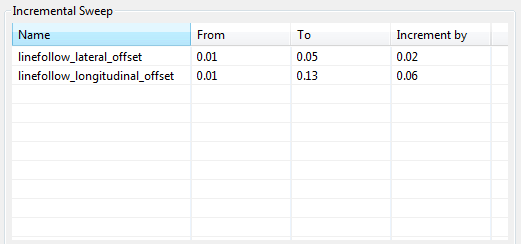
\includegraphics[width=.6\textwidth]{images/IncrementalSweep.png}
\caption{Incremental sweeping.\label{fig:IncrementalSweep}}
\end{figure}

\subsubsection{The value set Sweep}

In the first column it is possible to select from a drop-down the shared
design parameter to sweep (see Figure~\ref{fig:ValueSetSweep}). 
In the second column a list of double values
should be introduced, separated by (;).

\begin{figure}[htbp]
\centering
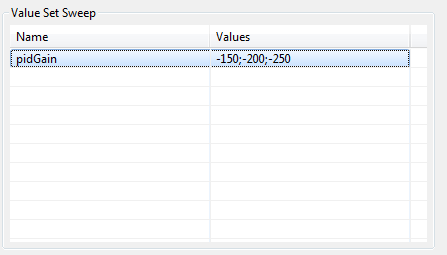
\includegraphics[width=.6\textwidth]{images/ValueSetSweep.PNG}
\caption{Selecting values of SDP variables to sweep over.\label{fig:ValueSetSweep}}
\end{figure}

It is possible to sweep by value set complex variables as shown in Figure~\ref{fig:ValueSetSweepComplex}.

\begin{figure}[htbp]
\centering
\includegraphics[width=.6\textwidth]{images/ValueSetSweepComplex.png}
\caption{Sweeping over complex variables.\label{fig:ValueSetSweepComplex}}
\end{figure}

The behaviour of complex SDPs is a bit different from the atomic SDPs.
For example, the configuration on the picture above will generate 2 ACA
runs for the variable ``\texttt{initial\_Position}''.

\begin{itemize}
\item 1st run: initial\_Position = {[}-1.448,-1.110{]}

\item 2nd run: initial\_Position = {[}-1.736,X*{]} - * where X is the value
defined in the base debug configuration for initional\_Position{[}2{]}.
\end{itemize}

The values defined in the value sweep are put together according to the
order they appear, if a for one of the indexes is missing (like in this
case the second value of initial\_Position{[}2{]}), the value from the
original debug configuration will be used.

\subsection{Scenario Tab}

In the scenarios tab it is possible to select which scenarios will be
used in the ACA run (see Figure~\ref{fig:ScenariosACATab}. 
The scenarios present in the ``\texttt{scenarios}'' folder
in the root of the project will be presented on the ``Scenario
selection'' table. It is then possible to check which scenarios will be
used in the ACA.

\begin{figure}[htbp]
\centering
\includegraphics[width=.6\textwidth]{images/ScenariosACATab.PNG}
\caption{Possibility for choosing multiple scenarios for ACA.\label{fig:ScenariosACATab}}
\end{figure}

\subsection{CT Settings Tab}

The CT side settings works in a similar fashion to the ones in
the normal
Crescendo launch (see Figure~\ref{fig:SettingsACATab}). 
The only difference is that it is possible to select
multiple options instead of one. In the ACA Settings tab it is only
possible to select options which have limited alternatives (i.e.,
enumerations).

\begin{figure}[htbp]
\centering
\includegraphics[width=.6\textwidth]{images/SettingsACATab.png}
\caption{Selecting CT Settings for ACA.\label{fig:SettingsACATab}}
\end{figure}

\subsection{Common Tab}

The common tab settings here work much in a similar fashion to the ones in
the normal
Crescendo launch (see Figure~\ref{fig:CommontabACA}). 

\begin{figure}[htbp]
\centering
\includegraphics[width=.6\textwidth]{images/CommontabACA.png}
\caption{Common tab for ACA.\label{fig:CommontabACA}}
\end{figure}

\section{Repeating a Single Launch Part of an ACA}

After a successful ACA launch, the \texttt{output} folder will contain
information regarding what was run in a specific ACA launch. Each ACA run has generated a file named \texttt{xxx.dlaunch}.

%This information in stored in the \texttt{output} folder. By looking at the result of an ACA run, it is possible to see a file named \texttt{xxx.dlaunch} for each ACA run.

By right-clicking a ``\texttt{.dlaunch}'' file and selecting the option
\emph{Crescendo} and then selecting the \emph{Create and Launch} option, 
the single selected run will
be launched again (see Figure~\ref{fig:CreateAndLaunchCommand}). 
This single launch configuration is also stored
together with the other launch configurations, typically its name is
prefixed by ``\texttt{generated}''.

\begin{figure}[htbp]
\centering
\includegraphics[width=.6\textwidth]{images/CreateAndLaunchCommand.png}
\caption{Relaunching single ACA experiments.\label{fig:CreateAndLaunchCommand}}
\end{figure}

By inspecting the launch configurations it is possible to find the launch
that was just created. The launch contains all the same settings as the
launch that was selected to be created from the ACA.

\begin{figure}[htbp]
\centering
\includegraphics[width=.6\textwidth]{images/GeneratedLaunch.png}
\caption{images/GeneratedLaunch.png}
\end{figure}

\section{Control Library}

In order to help build controllers in VDM that can handle low-level
proportional control in addition to supervisory control, a control
library has been included in the Crescendo tool. This library provides
classes that are equivalent to the \emph{P}, \emph{PD}, \emph{PI}
and \emph{PID} blocks of the 20-sim library under
\emph{Signal\textbackslash{}Control\textbackslash{}PID
Control\textbackslash{}Discrete}.

\subsection{Accessing the Control Library}

To use the control library, the class definitions must be imported into
the project.

\begin{itemize}
\item
  Right-click on the project and select \emph{New} and \emph{Other....}
\item
  Under the \emph{Crescendo folder}, select \emph{Add Crescendo
  Library~}and click~\emph{Next}.
\end{itemize}

\begin{figure}[htbp]
\centering
\includegraphics[width=.6\textwidth]{images/DestecsAddNewLibrary.png}
\caption{images/GeneratedLaunch.png}
\end{figure}

''Add the Control Library '\textbf{'TODO: New screenshot with control
library in.}

\begin{itemize}
\item
  Then check the box marked \emph{Control Library}.
\end{itemize}

Unless you want to edit the class files, leave ``Use linked libraries''
checked (default). The classes will now be added to your co-model.

\subsection{Using the Control Library}

\subsubsection{Basic Use}

To use a class from the library, simply define a variable of the correct
type, instantiate it with a constructor, call ``SetSampleTime'' and then
call ``Output'' in your control loop. All of the control library classes
have an operation called \emph{Output}, which takes in an error and
returns a control value, with the following form:

\begin{vdmrt}
public Output: real ==> real
Output(err) == ...

class Controller

instance variables

-- controller object
private pid: PID;

-- setpoint
private SP: real;

-- shared variables
private MV: real;
private out: real

operations
-- constructor for Controller
public Controller: () ==> Controller
Controller() ==
(
pid := new PID(10, 1, 0.1);
pid.SetSampleTime(SAMPLE_TIME)
);

-- control loop
public Step: () ==> ()
Step() ==
(
dcl err: real := SP - MV;
out := pid.Output(err)
);

-- 100Hz control loop
values SAMPLE_TIME = 0.01;
thread periodic(10E6, 0, 0, 0)(Step);

end Controller
\end{vdmrt}

Also, all of the classes have an operation called \emph{SetSampleTime},
which takes a sample time in seconds:

\begin{vdmrt}
public SetSampleTime: real ==> ()
SetSampleTime(s) ==
\end{vdmrt}

Unlike 20-sim, VDM does not have a \textbf{sampletime} keyword, so it is
necessary to explicitly tell the object what sample time to use in
calculations. Therefore, for all control objects (except P) you must
call \emph{SetSampleTime} before the ''Output ''is used. This only needs
to be done once and it is recommended that it is called immediately
after the constructor. If this is not done, the co-simulation will fail
with a pre-condition violation the first time \emph{Output} is called.

\subsection{Advanced Use}

All of the controller classes in the library are subclasses of a single
class called ``DTObject'' (Discrete-Time object). This class contains
the definitions for ``SetSampleTime'' and ``Output'' and enforces a
consistent interface. It is possible to use the various controller
classes without making reference to \emph{DTObject}. However, if it is
desirable to test different controllers, variables can be defined as
type \emph{DTObject}, meaning that only the call to the constructor
needs to be changed in order to use a different controller
implementation. This is also useful if control objects are passed to
controllers. In the following example, the \texttt{Controller} class can
accept any control object (\emph{P}, \emph{PID} etc.):

\begin{vdmrt}
class Controller

instance variables

-- controller object
private ctrl: DTControl;

operations

-- constructor for Controller
public Controller: DTControl ==> Controller
Controller(c) ==
(
ctrl := c;
ctrl.SetSampleTime(SAMPLE_TIME)
);

...
\end{vdmrt}

\subsection{Constructors}

\subsubsection{P}

The P class has the following constructors:

\begin{vdmrt}
-- set k
public P: real ==> P
P(k) == ...

-- default: k = 0.2
public P: () ==> P
P() == ...
\end{vdmrt}

\subsubsection{PD}

The PD class has the following constructors:

\begin{vdmrt}
-- set k, tauD, beta
public PD: real * real * real ==> PD
PD(k, tauD, beta) == ...

-- set k, tauD, beta = 0.1
public PD: real * real ==> PD
PD(k, tauD) == ...

-- default: k = 0.2, tauD = 1.0, beta = 0.1
public PD: () ==> PD
PD() == ...
\end{vdmrt}

\subsubsection{PI}

The PI class has the following constructors:

\begin{vdmrt}
-- set k, tauI
public PI: real * real ==> PI
PI(k, tauI) == ...

-- default: k = 0.2, tauI = 0.5
public PI: () ==> PI
PI() == ...
\end{vdmrt}

\subsubsection{PID}

The PID class has the following constructors:

\begin{vdmrt}
-- set k, tauI, tauD, beta
public PID: real * real * real * real ==> PID
PID(k, tauI, tauD, beta) == ...

-- set k, tauI, tauD, beta = 0.1
public PID: real * real * real ==> PID
PID(k, tauI, tauD) == ...

-- default: k = 0.2, tauI = 0.5, tauD = 0.5, beta = 0.1
public PID: () ==> PID
PID() == ...
\end{vdmrt}


\section{DE Architecture}\label{sec:DEArch}

This feature allows the selection of the hardware and deployment to be
specified in a separate file from the VDM system class.

In order to do this separation, the following steps need to be done:

\begin{itemize}
\item
  The System class must be cleaned of CPU and BUS~declarations and
  deployments of the objects
\item
  Annotations need to be added to the system class that indicate where
  the architecture and deployment statements.~The architecture tag must
  be places under an instance variables block:
\end{itemize}

\begin{vdmrt}
-- ## Architecture ## -- 
\end{vdmrt}

The deployment tab must be places in the constructor where the
deployment normally will have been specified:

\begin{vdmrt}
-- ## Deployment ## -- 
\end{vdmrt}

Architecture files (\texttt{.arch}), is placed in a folder called
"\texttt{model\_de/architectures}" in the project root. The
architecture files should have the following form:

\begin{vdmrt}
-- ## Architecture ## --
instance variables
cpu1: CPU := new CPU(<FCFS>, 1000000 /* Hz */);
cpu2: CPU := new CPU(<FCFS>, 1000000 /* Hz */);
cpu3: CPU := new CPU(<FCFS>, 1000000 /* Hz */);
bus1: BUS := new BUS(<FCFS>, 1000 /* bits/s */,{cpu1,cpu2,cpu3});
-- ## Deployment ## --
cpu1.deploy(mmi);
cpu3.deploy(navigation);
cpu2.deploy(radio);
\end{vdmrt}

When an architecture file like this is selected, the architecture and
deployment declaration is inserted in the ``right'' place (under the
tags in the \emph{system} file), creating a ``complete'' system just
before the co-simulation starts.

\section{Events}

Events can be triggered in the CT world. They will stop the simulation
before the allowed time slice is completed. The co-simulation engine
will then allow the DE simulator to take action but only until the point
where the event has been raised. The events are used in the contract in
order to support event-based triggering and not just time-triggered
scheduling.

\subsection{Simulation setup}

\subsubsection{Events in the contract}

For events to be considered during a simulation the event must be
defined in Section~\ref{sec:contract}:

\begin{grammar}
<events> ::= `event', <identifier>, `;'
\end{grammar}

\subsubsection{Events in the link file}

Events must be connected to a \texttt{\textbf{public async}} operation in VDM. This is
done by linking the event name specified in the contract to the fully
qualified operation name in VDM in the link file:

\begin{grammar}
<events> ::= 'event', <identifier> = 'System', '.', <identifier>, ('.', <identifier>)+
\end{grammar}

An example of this could be:

\begin{dcl}
event event1=System.eventHandler.event1;
\end{dcl}

Where:

\begin{itemize}
\item
  ``\texttt{event1}'' is the event name from the contract.
\item
  \texttt{System} is the \vdmkeyw{system} class.
\item
  \texttt{eventHandler} is the class holding the \texttt{\textbf{public async}} operation to execute.
\item
  ``\texttt{event1}'' (the last event1) is the \vdmkeyw{async} operation which to execute
  when the event occurs.
\end{itemize}

\subsection{Events in CT}

Events need to be marked using the keyword '\vdmkeyw{event}', this marks the
variable that it used as return value of the event function to be an
event variable. The keywords '\vdmkeyw{eventdown}' and 'eventup' are used as in
standalone 20-sim models. See more under Events. Example:

\begin{dcl}
variables
  boolean minLevelReached ('event');

equations
  maxLevelReached = eventup(levelIn-maxlevel);
\end{dcl}

\subsection{Events in DE}

The scheduler in VDM do not schedule events in the same way as for
instance a micro controller would do where the current executing job is
suspended in favour of the interrupt routine. However, it is possible to
get a similar behaviour by creating and deploying an object to a CPU
that contains the job to run when an interrupt occurs and then call this
from the \texttt{\textbf{async}} operation which is triggered when event occurs. It is
just important that no objects having a periodic threads are deployed to
the same CPU since this will delay the event by exactly one periodic
loop.

Events are linked to VDM through \vdmkeyw{async} operations and made assessable
through the \vdmkeyw{system} class.

\begin{vdmrt}
system System
instance variables
  eventHandler: EventHandler;
end System
\end{vdmrt}

The \vdmkeyw{async} operation must be specified in a class that is not deployed to
a CPU. This makes the evaluation instant. This means that the event
operation it self do not take time to run.

\begin{vdmrt}
class EventHandler

operations

public async event1: () ==> ()
event1()== skip;

end EventHandler
\end{vdmrt}

\textbf{Note about the VDM scheduler}: \emph{The VDM scheduler uses
priorities to select which thread should run, each thread is then
executed with a limited allowed number of expressions/statements it can
execute before another thread has to be schedulled and executed. The
priority defined how many expressions/statements a thread can execute
at a time. A thread will always continue executing until it is blocked
or finished the allowed number of expressions/statements.}

\chapter{Post-Analysis Possibilities}\label{chap:postana}

\section{Octave}\label{sec:octave}

GNU Octave is a high-level interpreted language, primarily intended for
numerical computations. It provides capabilities for the numerical
solution of linear and non-linear problems, and for performing other
numerical experiments. It also provides extensive graphics capabilities
for data visualization and manipulation. Octave is normally used through
its interactive command line interface, but it can also be used to write
non-interactive programs. The Octave language is quite similar to Matlab
so that most programs are easily portable.
\url{http://www.gnu.org/software/octave/}

\subsection{Octave Version}

It is very important that the correct version of Octave is used to run
the scripts generated by Crescendo. The correct version can be found in
Chessforge together with the Crescendo Releases.

\subsection{Octave use in Crescendo}

After each co-simulation run, an Octave script is generated in the
output dir. The script contains Octave code that reads the variable logs
produced by both VDM and 20-sim during the run.

\subsection{Show Plot Automatically when Script is Run}

There is one option available in the debug configuration that affects
the script. This option appears in two places both in the normal Crescendo
run and in ACA. If enabled, when the script is executed, a plot (or
several, depending on the amount of variables selected) will
automatically be drawn. In the case of an ACA run being executed, for
the same variable, the several runs will juxtaposed.

Figure~\ref{fig:octaveplotnormal} shows where to find this option for a normal run
(Post-Processing tab).

\begin{figure}[htbp]
\centering
\includegraphics[width=.6\textwidth]{images/TickOctaveplotNormal.png}
\caption{images/TickOctaveplotNormal.png}
\label{fig:octaveplotnormal}
\end{figure}

Figure~\ref{fig:octaveplotaca} show the ACA launch (Main Tab)

\begin{figure}[htbp]
\centering
\includegraphics[width=.6\textwidth]{images/TickOctavePlotACA.png}
\caption{images/TickOctavePlotACA.png}
\label{fig:octaveplotaca}
\end{figure}

\subsection{Invoking Octave from Crescendo}

It is possible to invoke Octave from the Crescendo IDE. Right-clicking on
an Octave (\texttt{.m}) file reveals the option ``Run Octave''. If you want to
use this command, be sure to tick the ``Show plot automatically when the
script runs'' box

\begin{figure}[htbp]
\centering
\includegraphics[width=.6\textwidth]{images/OctaveAction.png}
\caption{}
\end{figure}

If the option to show plot automatically was chosen, a plot will be drawn
and shown in a window like this:

\begin{figure}[htbp]
\centering
\includegraphics[width=.6\textwidth]{images/OctavePlotting.png}
\caption{}
\end{figure}

\subsection{Setting Octave path}

If your Octave installation was not made in the default installer path,
the path to Octave must be corrected in the Crescendo settings for the
feature mentioned above to work. The settings below can be found by
navigating to the Window-\textgreater{}Preferences menu.

\begin{figure}[htbp]
\centering
\includegraphics[width=.6\textwidth]{images/OctaveSettings.png}
\caption{images/OctaveSettings.png}
\end{figure}

\section{Folder Launch Configuration}

This is a new way of launching
an ACA by selecting a folder containing \texttt{.launch} files. The user has to
produce its own \texttt{.launch} files. The options to select are the project
and the folder containing the launch files. This is shown in Figure~\ref{fig:DirectoryLaunchMainTab}.

\begin{figure}[htbp]
\centering
\includegraphics[width=.6\textwidth]{images/DirectoryLaunchMainTab.png}
\caption{images/DirectoryLaunchMainTab.png}
\label{fig:DirectoryLaunchMainTab}
\end{figure}

\appendix
%%%% Bibliography %%%%
\newpage
\bibliographystyle{alpha}
\bibliography{dan}
\label{ch:bib} %label to refer to

\chapter{Glossary}\label{app:Glossary}

As might be expected in such an interdisciplinary project, terms and
concepts that are well known in one discipline may be unknown or
understood quite differently in another. This page therefore contains
common descriptions of core concepts agreed with the partners that are
used consistently within the project.

\begin{description}
\item[abstract class] (in object oriented programming) a class where one or more methods are defined abstractly using the text \textbf{\texttt{is subclass responsibility}} as their body.
\item[actuator] a component that produces a physical output in response to a signal~\cite{IEEE100}.
\item[aggregate] (in object oriented programming) the act of bringing together several objects into a single whole.
\item[automated co-model analysis] tool support for the selection of a single design from a set of design alternatives (including definition of scenarios, execution of co-simulations, and visualisation and analysis of co-simulation results).
\item[automated co-model execution] as automated co-model analysis except that is does not perform any analysis of the test results produced by the simulations
\item[bond] (in bond graphs) a directed point-to-point connection between power ports on submodels.  Represents the sharing of both \textit{flow} and \textit{effort} by those ports.
\item[bond graph] a domain independent idealised physical model based on the representing energy and its exchange between submodels.
\item[causality] (in bond graphs) dictates which variable of a power port is the input (cause) for submodel's equations and which is the output (effect).
\item[class] (in object oriented programming) the definition of the data field and methods an object of that class will contain.
\item[code generation] the process of implementing a system controller by automatically translating a model into a representation~(in some programming language) which can then be executed on the real hardware of the system.
%\item[commit] to record changes to data under revision control.
\item[co-model] a model comprising two constituent models (a DE submodel and a CT submodel) and a contract describing the communication between them.
%\item[configuration management] the managing of the composition of co-models from various DE and CT models.
\item[consistency] a co-model is consistent if the constituent models are both syntactically and semantically consistent.
\item[constituent model] one of the two submodels in a co-model.
\item[continuous-time simulation] a form of simulation where ``the state of the system changes continuously through time''~\cite[p.~15]{Robinson04}.
\item[contract] a description of the communication between the constituent models of a co-model, given in terms of shared design parameters, shared variables, and common events.
\item[controlled variable] a variable that a controller changes in order to perform control actions.
\item[controller] the part of the system that controls the plant.
\item[controller architecture] the allocation of software processes to CPUs and the configuration of those CPUs over a communications infrastructure.
\item[co-sim launch] the type of debug configuration used in the Crescendo tool to define and launch a single scenario.
\item[co-simulation baseline] the set of elements (co-model, scenario, test results etc.) required to reproduce a specific co-simulation.
\item[co-simulation engine] a program that supervises a co-simulation.
\item[co-simulation] the simulation of a co-model.
\item[cost function] a function which calculates the ``cost'' of a design.
\item[debug config] (Eclipse term) the place in Eclipse where a simulation scenario is defined.
\item[design alternatives] where two or more co-models represent different possible solutions to the same problem.
\item[design parameter] a property of a model that affects its behaviour, but which remains constant during a given simulation.
\item[design space exploration] the (iterative) process of constructing co-models, performing co-simulations and evaluating the results in order to select co-models for the next iteration.
\item[design step] a co-model which is considered to be a significant evolution of a previous co-model.
\item[discrete-event simulation] a form of simulation where ``only the points in time at which the state of the system changes are represented''~\cite[p.~15]{Robinson04}.
\item[disturbance] a stimulus that tends to deflect the plant from desired behaviour.
\item[edges] (in bond graphs) see \textit{bond}.
\item[effort] (in bond graphs) one of the variables exposed by a power port.  Represents physical concepts such as electrical voltage, mechanical force or hydraulic pressure.
\item[environment] everything that is outside of a given system.
\item[error] part of the system state that may lead to a failure~\cite{Avizienis&04}.
\item[event] an action that is initiated in one constituent model of a co-model, which leads to an action in the other constituent model.
\item[executable model] a model that can be simulated.
\item[failure] a system's delivered service deviates from specification~\cite{Avizienis&04}.
\item[fault injection] the act of triggering faulty behaviour during simulation.
\item[fault modelling] the act of extending a model to encompass faulty behaviours.
\item[fault] the adjudged or hypothesized cause of an error~\cite{Avizienis&04}.
\item[fault behaviour] a model of a component's behaviour when a fault has been triggered and emerges as a failure to adhere to the component's specification.
\item[fault-like phenomena] any behaviour that can be modelled like a fault (e.g.\ disturbance).
\item[flow] (in bond graphs) one of the variables exposed by a power port.  Represents physical concepts such as electrical current, mechanical velocity, fluid flow.
\item[ideal behaviour] a model of a component that does not account for disturbances.
\item[inheritance] (in object oriented programming) the mechanism by which a subclass contains all public and protected data fields and methods of its superclass.
\item[input] a signal provided to a model.
\item[interface] (in object oriented programming) a class which defines the signatures of but no bodies for any of its methods.  Should not be instantiated.
\item[junction] (in bond graphs) a point in a bond graph where the sum of flow (1-junction) or effort (0-junction) of all bonds to that point is zero.
\item[log] data written to a file during a simulation.
\item[metadata] information that is associated with, and gives information about, a piece of data.
\item[model base] the collection of artefacts gathered during a development (including various models and co-models; scenarios and test results; and documentation).
\item[model management] the activity of organizing co-models within a model base.
\item[model structuring] the activity of organizing elements within a model.
\item[model synthesis] see \textbf{code generation}.
\item[model] a more or less abstract representation of a system or component of interest.
\item[modelling] the activity of creating models.
\item[modularisation] construction of self-contained units (modules) that can be combined to form larger models.
\item[monitored variable] a variable that a controller observes in order to inform control actions.
\item[object] (in object oriented programming) an instantiation of a class, contains data fields and methods.
\item[objective function] see \textbf{cost function}.
\item[ontology] a structure that defines the relationships between concepts.
\item[operation] (in object oriented programming) defines an operation that an object may perform on some data.  Operations may be \emph{private, public} or \emph{protected}.
\item[output] the states of a model as observed during (and after) simulation.
\item[non-normative behaviour] behaviour that is judged to deviate from specification.
\item[physical concept] (in bond graphs) a class of component or phenomena that could exist or be observed in the real world, e.g. an electrical resistor or mechanical friction.
\item[plant] the part of the system which is to be controlled~\cite{IEEE100}.
\item[power port] (in bond graphs) the port type connected in a bond graph.  Contains two variables, \textit{effort} and \textit{flow}.  A power port exchanges energy with its connected models.
\item[private] (in object oriented programming, VDM) the method or data field may only be accessed from within the containing class.
\item[protected](in object oriented programming, VDM) the method or data field may only be accessed by its containing class or any of its subclasses.
\item[public] (in object oriented programming, VDM) the method or data field may be accessed by any other class.
\item[ranking function] a function that assigns a value to a design based on its ability to meet requirements defined by the engineer.
\item[realistic behaviour] a model of a component which includes disturbances defined by the tolerances associated with that component.
\item[repository] a shared store of data or files.
\item[response] a change in the state of a system as a consequence of a stimulus.
\item[revision control] the activity of managing changes (revisions) to computer data or files.
\item[scenario] test of a co-model.
\item[signal domain] where models share a single value or array at each port and where those ports are uni-directional, unlike bond graphs where the ports are bi-directional.
\item[sensor] a component whose input is a physical phenomenon and whose output is a quantitative measure of the phenomenon.
\item[shared design parameter] a design parameter that appears in both constituent models of a co-model.
\item[shared variable] a variable that appears in and can be accessed from both constituent models of a co-model.
\item[simulation] symbolic execution of a model.
\item[semantically consistent] the state when the constituent models of a co-model agree on the semantics of the varaibles, parameters and events they share.  The nature of these semantics is not yet described.
\item[static analysis] a method for checking some property of a model without executing that model.
\item[state event] an event triggered by a change within a model.
\item[stimulus] a phenomenon that effects a change in the state of a system.
\item[subclass] (in object oriented programming) a class that is defined as extending another class.  The other class becomes its superclass.  The subclass inherits all non private data fields and methods.
\item[submodel] a distinct part of a larger model.
\item[superclass] (in object oriented programming) the class from which a subclass is defined.
\item[syntactically consistent] the state when the constituent models of a co-model agree on the identities and data types of all shared variables, parameters and events.
\item[system boundary] the common frontier between a system and its environment.
\item[system under test~(SUT)] the part of a model that represents the system we wish to build, as opposed to parts of the model which are not part of this system.
\item[system] an entity that interacts with other entities, including hardware, software, humans and the physical world~\cite{Avizienis&04}.
\item[tag] to associate metadata with a piece of data.
\item[test result] a record of the output from a simulation of a model (see also \textbf{log}).
\item[time event] an expected event that occurs at a predetermined time.
\item[variable] part of a model that may change during a given simulation.
\item[vertices] (in bond graphs) the joining points of bonds.  May be manifested as either a \textit{junction} or a submodel.
\end{description} 

\end{document}
